\documentclass[cleveref]
{lipics-v2021}

\usepackage{microtype}
\usepackage{graphicx} % Required for inserting images
\usepackage{todonotes}
%\usepackage[disable]{todonotes} % author comments

\usepackage{amsthm} % theorem environments etc
\usepackage{amsfonts} % mathbb etc
\usepackage{amssymb} % symbols like \Rstriction
\usepackage{amsmath} % align etc
\usepackage{xspace} % spaces after commands without braces
\usepackage{mathtools} % coloneqq etc
\usepackage{booktabs}
% \usepackage{enumitem}
\usepackage{hyperref}
\usepackage{tabularx}

\hideLIPIcs
\nolinenumbers
\bibliographystyle{plain}

%\title{Complexity of logics and semiring semantics}
\title{Logic and Computation Through the Lens of Semirings}
%\title{Logic and Complexity Through the Lens of Semirings}
%\author{Joan R. Public\footnote{Optional footnote, e.g. to mark corresponding author}}{Department of Informatics, Dummy College, [optional: Address], Country}{joanrpublic@dummycollege.org}{[orcid]}{[funding]}
\author{Timon Barlag}{Leibniz University Hannover, Germany}{barlag@thi.uni-hannover.de}{https://orcid.org/0000-0001-6139-5219}{}
\author{Nicolas Fröhlich}{Leibniz University Hannover, Germany}{nicolas.froehlich@thi.uni-hannover.de}{https://orcid.org/0009-0003-5413-1823}{Appreciates funding by the German Research Foundation (DFG) under the project id ME4279/3-1.}
\author{Teemu Hankala}{University of Helsinki, Finland}{teemu.hankala@helsinki.fi}{}{}
\author{Miika Hannula}{University of Tartu, Estonia and University of Helsinki, Finland}{miika.hannula@ut.ee}{https://orcid.org/0000-0002-9637-6664}{Partially supported by the European Research Council (ERC)
under the European Union’s Horizon 2020 research and innovation programme (grant
agreement No 101020762).}
\author{Minna Hirvonen}{University of Helsinki, Finland}{minna.hirvonen@helsinki.fi}{https://orcid.org/0000-0002-2701-9620}{This project has received funding from the European Research Council (ERC)
under the European Union’s Horizon 2020 research and innovation programme (grant
agreement No 101020762).}
\author{Vivian Holzapfel}{Leibniz University Hannover, Germany}{holzapfel@thi.uni-hannover.de}{https://orcid.org/0009-0001-1439-5037}{}
\author{Juha Kontinen}{University of Helsinki, Finland}{juha.kontinen@helsinki.fi}{https://orcid.org/0000-0003-0115-5154}{Supported by grants 359650 and 345634 of the Academy of Finland.}
\author{Arne Meier}{Leibniz University Hannover, Germany}{meier@thi.uni-hannover.de}{https://orcid.org/https://orcid.org/0000-0002-8061-5376}{Appreciates funding from the DAAD (Deutscher Akademischer Austauschdienst = German Academic Exchange Service) project-id 57710940 as well as from the German Research Agency (DFG) under the project-id ME 4279/3-1}
\author{Laura Strieker}{Leibniz University Hannover, Germany}{strieker@thi.uni-hannover.de}{https://orcid.org/0009-0005-4878-4953}{}




\date{February 2025}
%\Copyright{Jane Open Access and Joan R. Public} %TODO mandatory, please use full first names. LIPIcs license is "CC-BY";  http://creativecommons.org/licenses/by/3.0/
\Copyright{Timon Barlag, Nicolas Fröhlich, Teemu Hankala, Miika Hannula, Minna Hirvonen, Vivian Holzapfel, Juha Kontinen, Arne Meier, and Laura Strieker}
\authorrunning{T. Barlag et al.}

\ccsdesc[500]{Theory of computation~Abstract machines}
\ccsdesc[500]{Theory of computation~Turing machines}
\ccsdesc[300]{Theory of computation~Verification by model checking}
\ccsdesc[100]{Theory of computation~Circuit complexity}
\ccsdesc[100]{Theory of computation~Complexity classes}
%mandatory: Please choose ACM 2012 classifications from https://dl.acm.org/ccs/ccs_flat.cfm 

\keywords{Semiring, Provenance, FO, BSS Machines, Turing Machines, Computational Complexity, Circuit Complexity} %TODO mandatory; please add comma-separated list of keywords



% \theoremstyle{plain}
% \newtheorem{theorem}{Theorem}[section]
% \newtheorem{lemma}[theorem]{Lemma}
% \newtheorem{proposition}[theorem]{Proposition}
% \newtheorem{corollary}[theorem]{Corollary}

% \theoremstyle{definition}
% \newtheorem{definition}[theorem]{Definition}
% \newtheorem{example}[theorem]{Example}
% \newtheorem{observation}[theorem]{Observation}
% \theoremstyle{remark}
% \newtheorem{remark}[theorem]{Remark}

% author commands
% author colors
\newcommand{\timoncolor}{brown!20}
\newcommand{\juhacolor}{red!20}
\newcommand{\lauracolor}{green!20}
\newcommand{\viviancolor}{purple!20}
\newcommand{\minnacolor}{teal!20}
\newcommand{\nicolascolor}{blue!20}
\newcommand{\teemucolor}{magenta!20}
\newcommand{\miikacolor}{orange!20}

\newcommand{\todoi}[1]{\todo[inline]{#1}}
 
% author inline commands
\newcommand{\timon}[1]{\todo[inline, size=\small, color=\timoncolor]{Timon: #1}}
\newcommand{\juha}[1]{\todo[inline, size=\small, color=\juhacolor]{Juha: #1}}
\newcommand{\laura}[1]{\todo[inline, size=\small, color=\lauracolor]{Laura: #1}}
\newcommand{\vivian}[1]{\todo[inline, size=\small, color=\viviancolor]{Vivian: #1}}
\newcommand{\minna}[1]{\todo[inline, size=\small, color=\minnacolor]{Minna: #1}}
\newcommand{\nicolas}[1]{\todo[inline, size=\small, color=\nicolascolor]{Nicolas: #1}}
\newcommand{\teemu}[1]{\todo[inline, size=\small, color=\teemucolor]{Teemu: #1}}
\newcommand{\miika}[1]{\todo[inline, size=\small, color=\miikacolor]{Miika: #1}}
\newcommand{\arne}[2][]{\todo[size=\small, textcolor=white,linecolor=green!50!black,bordercolor=green!50!black,backgroundcolor=green!50!black,#1]{{\sffamily Arne: #2}}}

% author margin commands
\newcommand{\timonS}[1]{\todo[size=\tiny, color=\timoncolor]{Timon: #1}}
\newcommand{\juhaS}[1]{\todo[size=\tiny, color=\juhacolor]{Juha: #1}}
\newcommand{\lauraS}[1]{\todo[size=\tiny, color=\lauracolor]{Laura: #1}}
\newcommand{\vivianS}[1]{\todo[size=\tiny, color=\viviancolor]{Vivian: #1}}
\newcommand{\minnaS}[1]{\todo[size=\tiny, color=\minnacolor]{Minna: #1}}
\newcommand{\nicolasS}[1]{\todo[size=\tiny, color=\nicolascolor]{Nicolas: #1}}
\newcommand{\teemuS}[1]{\todo[size=\tiny, color=\teemucolor]{Teemu: #1}}

%\logics
\newcommand{\arb}{\mathrm{Arb}_K}
\newcommand{\arbF}{\mathrm{Arb}_K}
\newcommand{\enc}{\textit{enc}}
\newcommand{\lit}{\textit{Lit}}
\newcommand{\logicFont}[1]{\protect\ensuremath{\mathrm{#1}}\xspace}
\newcommand{\FOK}{\ensuremath{{\logicFont{FO}}_{K}}\xspace}
\newcommand{\FO}{\ensuremath{{\logicFont{FO}}}\xspace}


% misc/math commands
\newcommand{\R}{\mathbb{R}}
\newcommand{\C}{\mathbb{C}}
\newcommand{\N}{\mathbb{N}}
\newcommand{\ol}{\overline}
\newcommand{\bO}{\mathcal{O}}
\newcommand{\ar}{\ensuremath{\textnormal{ar}}\xspace}
\newcommand{\nnf}{\ensuremath{\textnormal{nnf}}\xspace}
\newcommand{\ddfn}{\Coloneqq}
\newcommand{\dfn}{\coloneqq}

% BSS commands
\newcommand{\BSSK}{\mathrm{BSS}_K}
\newcommand{\PK}{\mathrm{P}_K}
\newcommand{\LTK}{\mathrm{LT}_K}

% circuit commands
\newcommand{\calC}{\mathcal{C}}
\newcommand{\ACO}{\mathrm{AC}^0_{K}}
\newcommand{\FACO}{\mathrm{FAC}^0_{K}}
\newcommand{\size}{{\mathrm{size}}}
\newcommand{\depth}{{\mathrm{depth}}}
\newcommand{\unip}{\mathrm{U}_{\PK}}
\newcommand{\unil}{\mathrm{U}_{\LTK}}

% problem environments
\usepackage{booktabs}
\newcommand{\decproblemdef}[3]{%
\begin{center}
\begin{tabular}{lp{10cm}}\toprule
\textsf{\bfseries Problem:}& #1 \\\midrule
\textsf{\bfseries Input:}& #2\\
\textsf{\bfseries Question:}& #3?\\\bottomrule
\end{tabular}
\end{center}
}

\newcommand{\fv}{\mathrm{FV}}

\newcommand{\funcproblemdef}[3]{%
\begin{center}
\begin{tabular}{lp{9cm}}\toprule
\textsf{\bfseries Problem:}& #1 \\\midrule
\textsf{\bfseries Input:}& #2\\
\textsf{\bfseries Output:}& #3\\\bottomrule
\end{tabular}
\end{center}
}

% problem definitions
\newcommand{\EVAL}{\text-\mathrm{EVAL}}
\newcommand{\MC}{\text-\mathrm{MC}}
\newcommand{\FOKMC}[2][O]{\FOK(#1)\MC\def\temp{#2}\ifx\temp\empty\else_#2\fi}

% eval brackets
\usepackage{stmaryrd}
\newcommand{\evaluate}[2]{\protect\ensuremath{\llbracket#1\rrbracket_{#2}}}

% Tikz
\usepackage{tikz}
\usetikzlibrary{
    arrows,
    positioning,
}

% Algorithms
\usepackage[linesnumbered, ruled, vlined]{algorithm2e}
\newcommand{\procEval}{{\normalfont\texttt{Eval}}}

% Complexity classes
\newcommand{\PSPACEK}{\mathsf{PSPACE}_K}


\newcommand{\ourpar}[1]{%
  \par\vspace{\baselineskip}%
  \noindent\textbf{\sffamily #1. }%
}


\begin{document}



\maketitle
\begin{abstract}
We study computational aspects of first-order logic and its extensions in the semiring semantics developed by Gr\"adel and Tannen. 
We characterize the complexity of model checking and  data complexity of first-order logic  both in terms of a generalization of BSS-machines and arithmetic circuits defined over $K$. 
In particular, we give a logical characterization of  $\FACO$ by an extension of first-order logic that holds for any $K$ that is both commutative and positive. 
\end{abstract}

%\teemu{Can we fit the title on a single line? Computation vs. complexity ($\leftarrow$ does not fit either) or something else?}
%\teemu{Oxford/Non-Oxford British English / American English? Australian?}
%\arne[inline]{good point, Teemu. I would be in favour of UK English}
\section{Introduction}
In the last decade, the use of semirings to study provenance has attracted more attention~\cite{gradel17semiringprovenancefirstordermodel,DannertGNT21,DBLP:conf/lics/GradelHNW22,abs-1712-01980,GreenKT07}.
In this article, we study computational aspects of first-order logic in the semiring semantics originating from the study of provenance in databases~\cite{GreenKT07}.

Semirings are algebraic structures that generalize rings by relaxing the requirement for additive inverses. 
They have found numerous applications in computer science due to their versatility and modularity in modeling and analyzing computational problems~\cite{DBLP:journals/fuin/RudeanuV04,DBLP:journals/tcs/Peeva91,DBLP:journals/ijac/GaubertK06,DBLP:journals/soco/LitvinovRSS13,DBLP:journals/cj/Moller13,DBLP:journals/ijfcs/EsparzaLS15,DBLP:journals/order/Vrana22}.
In other words, specific semirings correspond to different computational paradigms or problem domains. Important examples of semirings include the \emph{Boolean semiring} $\mathbb{B}=(\mathbb{B},\lor,\land,0,1)$ as the simplest example of a semiring that is not a ring, the \emph{probability semiring} $\mathbb{R}_{\geq 0}=(\mathbb{R}_{\geq 0},+,\cdot,0,1)$ consisting of the non-negative reals with standard addition and multiplication, and the \emph{semiring of natural numbers} $\mathbb{N}=(\mathbb{N},+,\cdot,0,1)$ which consists of natural numbers with their usual operations.
Yet, other examples include the semiring of multivariate polynomials $\mathbb{N}[X]=(\mathbb{N}[X],+,\cdot,0,1)$ which is the free commutative semiring generated by the indeterminates in $X$,  the \emph{tropical semiring} $\mathbb{T} = (\mathbb{R}\cup\{\infty\}, \min, +, \infty, 0)$ which consists of the reals expanded with infinity	and has $\min$ and $+$ respectively plugged in for addition and multiplication, and the \L{}ukasiewicz semiring $\mathbb{L} = ([0,1], \max, \cdot , 0, 1)$, used in multivalued logic, which endows the unit interval with $\max$ addition and multiplication $a \cdot b \dfn \max(0, a+b-1)$.

Most of the classical complexity theory lives in the domain of the Boolean semiring $\mathbb{B}$, whereas $\mathbb{N}$ is the domain of problems related to counting, and $\mathbb{R}_{\geq 0}$ for problems with geometric or continuous features. 
On the other hand, tropical semirings have various applications in performance analysis~\cite{DBLP:journals/access/OmanovicOC23} and reachability problems~\cite{DBLP:journals/ijac/GaubertK06}.

Several computation models can be generalized to various classes of semirings. 
For example, weighted automata and weighted Turing machines label the transitions of the machine with semiring elements representing quantities such as probabilities, costs, or capacities. 
Different semirings enable automata to model varied quantitative behaviours with a wide array of applications (see, e.g., \cite{KOSTO,badia}). 
Furthermore, circuit complexity theory and algebraic algorithms readily generalize to various families of semirings (see \cite{ganardi} and the references therein).    

Semirings have also found applications in database query evaluation. 
Semiring provenance is an approach to query evaluation in which the result of a query is something more than just mere one-bit true/false answer. 
The basic idea behind this approach is to annotate the atomic facts in a database by values from some semiring $K$, and to propagate these values through a query.
Depending on the choice of the semiring, the provenance valuation gives information about a query, e.g., regarding its confidence, cost, or the number of assignments that make the query true \cite{GreenKT07}.
Semiring semantics for query languages is currently an actively studied topic in database theory (see, e.g.,
 \cite{10.1145/3651146,im_et_al:LIPIcs.ICDT.2024.11} for Datalog queries and  \cite{eldar_et_al:LIPIcs.ICDT.2024.4,munozserrano_et_al:LIPIcs.ICDT.2024.12,tencate_et_al:LIPIcs.ICDT.2024.8} for conjunctive queries). 

Semiring semantics has also been defined for first-order logic \cite{abs-1712-01980,Tannen17}. In this context, it has particularly been explored via key themes in classical finite model theory, including Ehrenfeucht--Fra\"{i}ss\'{e} games, locality, 0-1 laws, and definability up to isomorphisms \cite{BiziereGN23,BrinkeGM24,GradelHNW22, GradelM21}.
Recently, semiring semantics has been further extended to more expressive logical languages such as fixed-point logic \cite{DannertGNT21} and team-based logics \cite{BarlagHKPV23}.  
It is worth noting that the logics in these works differ from the logics studied in the context of weighted machines and logics \cite{KOSTO,badia}. 
In fact, a natural
computation model for our purposes is a generalization of the BSS-machine that we  define in this article. The inputs of such a machine are  finite sequences of the elements of the semiring $K$ whereas the weighted machines  operate with classical Boolean inputs.


\ourpar{Contributions}
In order to characterize the complexity of model checking, we generalize the well-known BSS-machines~\cite{BSSbook} to arbitrary semirings. 
We also give a logical characterisation of (non-uniform) $\FACO$ by an extension of first-order logic that is true for any semiring~$K$ that is commutative and positive. 


\ourpar{Organisation}
In Section~\ref{BSS}, we generalize the BSS-model from the reals to a wide variety of  semirings and show how classical computations can be simulated on such a machine. 
In Section~\ref{Circuits}, we go through the basic definitions regarding arithmetic circuits over a semiring. 
In Section~\ref{logic}, we define the semiring interpretation of first-order formulas. In Section~\ref{results}, 
we characterize the complexity of model checking and the data complexity of first-order logic over a semiring $K$ in terms of a generalization of BSS-machines and in Section~\ref{circ} we give a characterization via arithmetic circuits defined over~$K$. 


% \miika{I removed this citation \cite{10.1145/3651596} which concerns instance-based (as opposed to tuple-based) provenance with first-order logic; it was mentioned that this paper defined semiring semantics for first-order logic with negation, but I think this was done for the first time by grädel and tannen.}



\section{Preliminaries}
% \vivian{I finish this section}
% \vivian{add one example for section}
We assume familiarity with basic concepts in theoretical computer science, e.g., Turing machines~\cite{DBLP:books/daglib/0086373}. 
We start with the fundamental definition of a semiring.
\begin{definition}
    A \emph{semiring} is a tuple $K=(K,+,\cdot,0,1)$, where $+$ and $\cdot$ are binary operations on $K$, $(K,+,0)$ is a commutative monoid with identity element $0$, $(K,\cdot ,1)$ is a monoid with identity element $1$, $\cdot$ left and right distributes over $+$, and $x \cdot 0 =0= 0\cdot x$ for all $x \in K$.
    $K$ is called \emph{commutative} if $(K,\cdot ,1)$ is a commutative monoid.
    As usual, we often write $ab$ instead of $a \cdot b$. 

    A semiring is \emph{ordered} if there exists a partial order $\leq$ such that for all $a,b, c \in K$ $a\leq b \implies a+c \leq b+c$ and $0\leq a, 0 \leq b \implies 0 \leq ab$.

    A semiring is \emph{positive} if it has no divisors of $0$, i.\,e. $ab\neq 0$ for all $a,b\in K$, where $a\neq 0 \neq b$ and if $a+b=0$ implies that $a=b=0$.
\end{definition}

Throughout this paper, we only consider nontrivial semirings, i.e., semirings where $0 \neq 1$.

%\timon{We probably need/want commutative semirings everywhere, right?}
%\miika{It seems positivity of $K$ is assumed everywhere; state it here and omit in the sequel?}

\subsection{\texorpdfstring{BSS$_K$}{BSSK} Machines}\label{BSS}

% \todoi{Todo: Fill in gaps in definitions etc in this seciton. Mostly use the the BSS book as reference and adjust for semirings.}

%\timon{mention: only infinite semirings?}

%\teemu{%Some things that are still missing and that someone (anyone) should probably write some poetry about:
%%(1)
%The following should probably be given at least some answer:
%What BSS machines mean in general and why are we using them? Why go through all the trouble instead of
%using (extended) Turing machines right away?
%%(2) Something general about the meaning of the tape and the shift operations, even if these
%%are probably known to the main audience. In particular, explain the meaning of the dot
%%in the notation.
%}

\begin{definition}
%    For a positive semiring $K$ we define $K^* = \bigcup_{n\geq 0} K^n$ and $K_*$ as the set of all $x$ of the form $x= (\dots,x_{-2}, x_{-1}, x_0 \textbf{.} x_1, x_2, \dots)$ where $x_i \in K$ for all $i \in \mathbb{Z}$ and for a sufficiently large $k$, all $x_j=0$ with $|j| \geq k$.  
    For a semiring $K$ we define $K^* = \bigcup_{n\geq 0} K^n$ and denote by $K_*$ the set of all $x$ of the form $x= (\dots,x_{-2}, x_{-1}, x_0 \textbf{.} x_1, x_2, \dots)$, where $x_i \in K$ for all $i \in \mathbb{Z}$ and for some sufficiently large $k$, it holds that $x_j=0$ for all $j$ with $|j| \geq k$.  
\end{definition}
%\juha{Explain the dot between $x_0$ and $x_1$ in the above definition}

\begin{definition}
   % We define two shift operations on $K_*$. Shift left $\sigma_l$, where $\sigma_l(x)_i = x_{i+1}$ and its inverse shift right $\sigma_r$, where $\sigma_r(x)_i = x_{i-1}$.  
     We define two shift operations on $K_*$. Shift left $\sigma_l$, where $\sigma_l(x_i) = x_{i+1}$ and its inverse shift right $\sigma_r$, where $\sigma_r(x_i) = x_{i-1}$.  
\end{definition}

%\teemu{I think that the definition of BSS$_K$ machines makes sense for every semiring with $0 \neq 1$.
%The Boolean semiring with two elements yields a machine that is (at least in some sense) just an alternative version of a Turing machine.}
%\timon{I agree. I added a sentence below the semiring definition stating that we only consider nontrivial semirings.}

%\miika{Added below paragraph}
The following definition adapts BSS machines to arbitrary semirings $K$. The computation nodes of a BSS machine are usually formulated in terms of quotients of polynomial functions with real coefficients. Since semirings generally lack additive and multiplicative inverses, BSS$_K$ machines have no operations corresponding to subtraction and division.  
\begin{definition}[BSS$_K$ machines] \label{def:BSSK} 
    Let $K$ be a
    %positive
    %, ordered
    semiring. 
    A BSS$_K$ machine consists of an input space $\mathcal{I}=K^*$, a state space $\mathcal{S}=K_*$ and an output space $\mathcal{O}=K^*$, together with a
    %connected
    directed graph whose nodes are labelled by $1, \ldots, N$. 
    The nodes are of five different types.
    %
    \begin{itemize}
        \item \emph{Input node}. The node labelled by $1$ is the only input node. The node is associated with a next node $\beta(1)$ and the input mapping $g_I\colon \mathcal{I} \to \mathcal{S}$.
        \item \emph{Output node}. The node labelled by $N$ is the only output node. This node is not associated with any next node. 
        Once this node is reached, the computation halts, and the result of the computation is placed on the output space by the output mapping $g_O\colon \mathcal{S}\to \mathcal{O}$.
        \item \emph{Computation nodes.} A computation node $m$ is associated with a next node $\beta(m)$ and a mapping $g_m\colon \mathcal{S}\to \mathcal{S}$ such that for some $c \in K$ and $i,j,k\in \mathbb{Z}$ the mapping $g_m$ is identity on coordinates $l \neq i$ and on coordinate $i$ one of the following holds:
        %
        \begin{itemize}
            \item $g_m(x)_i =x_j+x_k$ (addition),
            \item $g_m(x)_i = x_j\times x_k$ (multiplication),
            \item $g_m(x)_i = c$ (constant assignment).
        \end{itemize} 
        \item \emph{Branch nodes.} A branch node $m$ is associated with nodes $\beta^-(m)$ and $\beta^+(m)$. 
        Given $x\in \mathcal{S}$ the next node is $\beta^-(m)$ if $x_1 = x_2$ and $\beta^+(m)$, otherwise. 
        If $K$ is ordered, instead the next node is $\beta^-(m)$ if $x_1 \leq x_2$ and $\beta^+(m)$, otherwise.
%        \teemu{Is this in the middle of changes? If the latter one is intended to be $\leq$, we
%        would need to have separate programming for ordered and unordered cases. (It wouldn't matter much, though.)}
%        \timon{Yeah, it was supposed to be $\leq$. Since we can simulate $=$ via $\leq$}
        % \nicolasS{allow comparison with constant?}
        % \teemu{Would it be better to let $x_0 = 0$ and $x_0 = x_1$ (or something similar) be the basic branching conditions and
        % include $x_0 \leq x_1$ (or $x_i \leq x_j$) for those structures that have the relation $\leq$
        % defined?}
        % \vivian{if we  use ordered semirings isn't $\leq$ then always defined?}
        \item \emph{Shift nodes.} A shift node $m$ is associated either with shift left $\sigma_l$ or shift right $\sigma_r$, and a next node $\beta(m)$.
    \end{itemize}
    %
    The input mapping $g_I\colon \mathcal{I} \to \mathcal{S}$ places an
    input $(x_1, \ldots ,x_n)$ in the state
    \[
        (\ldots , 0, \underbrace{1, \dots, 1}_{n}, 0\textbf{.} x_1, \ldots ,x_n, 0,\ldots )\in \mathcal{S},
    \]
    where the size of the input $n$ is encoded in unary in the $n$ first negative coordinates.
    The output mapping $g_O\colon \mathcal{S}\to \mathcal{O}$ maps a state to the string consisting of its first $l$ positive coordinates, where $l$ is the number of consecutive ones stored in the negative coordinates starting from the first negative coordinate.
   
    A configuration at any moment of computation consists of a node $m\in \{1, \ldots ,N\}$ and a current state $x\in\mathcal{S}$.
    The (sometimes partial) \emph{input-output} function $f_M \colon K^*\to K^*$ of a machine $M$ is now defined in the obvious manner.
    A function $f \colon K^*\to K^*$ is \emph{computable} if $f=f_M$ for some machine $M$. A language $L \subseteq K^*$ is \emph{decided} by a BSS$_K$ machine $M$ if its characteristic function $\chi_L \colon K^* \to K^*$ is $f_M$. 
\end{definition}

\begin{example}
For instance, $g_O$ maps 
\[
    (\ldots ,2,1,1,1,0\textbf{.}x_1, x_2,x_3,x_4,\ldots )\in \mathcal{S},
\]
to $(x_1, x_2,x_3)\in \mathcal{O}$.
\end{example}

% \paragraph*{Deterministic complexity classes.}
    % TIMESPACE for $BSS_K$, also $P_K$, maybe $NP_K$?
\begin{definition}
    A machine $M$ \emph{runs in (deterministic) time} $t\colon \N \rightarrow \N$, if $M$ reaches the output in $t(|x|)$ steps for each input $x\in \mathcal{I}$.
    The machine $M$ runs in \emph{polynomial time} if $t$ is a polynomial function.
    The complexity class $\PK$ is defined as the set of all subsets of $K^*$ that are decided by some machine $M$ running in polynomial time. 
\end{definition}
\begin{definition} 
    A machine $M$ \emph{requires space} $s\colon \N \rightarrow \N$, if $M$ reaches the output using $s(|x|)$ coordinates of the state space for each input $x\in \mathcal{I}$.
    The machine $M$ requires \emph{polynomial space} if $s$ is a polynomial function.
    The complexity class $\PSPACEK$ is defined as the set of all subsets of $K^*$ that are decided by some machine $M$ requiring polynomial space. 
\end{definition}

% \begin{definition}
%     \todo[inline]{Some sort of tape normal form, where in between each two ``useful'' cells, there is a cell containing a $1$.
%     This is useful, to be able to do arbitrary comparisons at any point of the computation and to ``carry'' values along the tape.}
% \end{definition}

Arbitrary computations and comparisons need a way to remember intermediate values.
To this end, we use $(\dots, 0\textbf{.}\, x_1, 1, x_2, 1 \dots, x_n, 1, 0 \dots)$ as a more useful starting state of a BSS$_K$ machine.
The gap between two input values allows the machine to temporarily store values or move a value from one end of the state space to the other.
The following result shows, that obtaining this \emph{gap normal form} can be achieved with polynomial
%\teemuS{This (minimal) needs to be changed?}\nicolasS{changed to polynomial}
overhead as an initialization step of a BSS$_K$ machine.

%\teemu{Does the following result have a similar inverse operation? Is it linear? Then
%we could add some handwaving to say that we could instead (modulo linear time) consider machines with the
%operations mentioned in remark~\ref{remark:comparisons} without having to think about the simulation
%during the actual computation.}
%\nicolas{I think the idea was to use this normal form to justify remark~\ref{remark:comparisons}, because $x_i = x_j$ and especially $x_i = c$ can be easily realized using the gaps.
%I would assume the inverse is also doable, but I have no concrete idea.}
%\teemu{Being able to test for $x_1 = 0$ would be nice for the output phase.}
%\teemu{Edit: I may have a fix for the problem I had with this.}

\begin{proposition}\label{prop:gap}
    The initial state space $(\dots, 0, 1, \ldots, 1, 0\textbf{.} x_1, \ldots ,x_n, 0,\ldots )$ can be converted into $(\dots, 0\textbf{.}\, x_1, 1, x_2, 1 \dots, x_n, 1, 0 \dots)$ with quadratic overhead.
    Similarly, the reverse direction can be achieved with quadratic overhead.
\end{proposition}
%\teemu{I try to make a sketch for the reverse direction in the appendix. It would be great,
%if someone would be able to check it and possibly make some polishing as well.}
%\nicolas{how important is the inverse procedure? I think it would be fine to hand-wave their existence, otherwise I could construct another machine if you want. I believe you can mostly reverse the current machine.}
%\teemu{If there is some way that we can be confident about, it would be nice. Otherwise we
%would have to change the result concerning Turing machines (not able to use the official
%output format of BSS machines) or change the definition of BSS machines to allow
%testing for $x_1 = 0$ (which would render the normal form more or less obsolete).
%(EDIT: not obsolete, since there are still comparisons $x_i = x_j$, but these are not
%necessary for the Turing machine simulation.)
%(Other constants are not needed in the comparisons.) If we are only interested in outputs of length one,
%then none of this matters, as that case is easy. It might also be possible to use the
%Turing machine without going first for the gap normal form, but when I tried to do it this way,
%it did not really seem any easier (?).}
%\nicolas{Ok. I will think about the reverse direction.}
%\teemu{Alternatively, it is also possible to change the Turing simulation so that instead of
%computing a function $f \colon K^* \to K^*$ we would have $f \colon K^* \to K^n$ for
%a fixed $n \in \mathbb N$.}
%\nicolas{I added a machine for the reverse direction into the appendix}
%\teemu{Great!}
\begin{proof}
Figure~\ref{fig:bss normal form machine} in Appendix~\ref{appendix} implements the subroutine \texttt{Init}, converting the initial configuration into $(\dots, 0\textbf{.}\, x_1, 1, x_2, 1 \dots, x_n, 1, 0 \dots)$ in $\bO(n^2)$ steps.
Analogously, Figure~\ref{fig:bss normal form machine reverse} implements the reverse. 
\end{proof}

\begin{remark}\label{remark:comparisons}
    Using the gap normal form allows easy simulation of branching nodes using $x_i = x_j$ or $x_i = c$ as branching condition.
\end{remark}

%\teemu{Add a (very) short definition for extended BSS machines with the operations in remark %\ref{remark:comparisons} using a tape of the form $(\{0, 1\}^2)_*$. Note that these machines
%now have a blank symbol that is not part of the intended input alphabet.}

%\teemu{Does anyone else besides me need the following lemma? I am considering to make it
%just a small part of result about Turing machines.}
%
%\begin{lemma}
%Let $M$ be a machine that is otherwise similar to a BSS$_K$ machine but extended with a finite
%set $Q$ of states, one state being active at any step of the computation, starting with
%an initial state $q_0 \in Q$, and allowing machine instructions of the following two forms:
%(i) set the internal state of the machine to some fixed $q \in Q$; (ii)
%branch on the internal state $q$ of the machine, i.e., $\beta(m) = \delta_m(q)$ for some fixed
%function $\delta_m$. Then, there is an ordinary BSS$_K$ machine that on any input proceeds
%tape-wise exactly as the machine $M$ at each step of the computation.
%\end{lemma}
%
%\begin{proof}
%The states of the set $Q$ can be encoded in the machine instructions of a new machine $M'$:
%for each of the nodes $i \in [N]$ and states $q \in Q$ there is a node for $(i, q)$,
%with the following exceptions: for the initial node $1$ only $(1, q_0)$ is needed, and
%the output nodes $(N, q)$ can be joined together (e.g.{} to $(N, q_0)$).
%The ordinary branch nodes of the machine preserve the added state, and when branching on state
%of the machine, the next node is given by the associated function (and state is preserved).
%\end{proof}
%
%\begin{lemma}
%Let $k \in \mathbb N$ be fixed. Then the following subroutines take a constant amount of time.
%\begin{enumerate}
%\item[(i)] $k$-shift left and $k$-shift right
%\item[(ii)] Branching based on a first-order definable (i.e., a Boolean combination of facts) Boolean query on elements $x_0, \dots, x_{k - 1}$
%\timon{first-order or propositionally definable?}
%\teemu{Well, while writing this I was just thinking about using the indices directly.
%Then, quantifiers don't really add anything new.}
%using the comparisons allowed by the machine.
%\miika{What if the Boolean query encodes SAT? I am misreading this somehow(?)}
%\teemu{We are using the fixed elements $x_0, \dots, x_{k - 1}$ (or $x_1, \dots, x_k$ if that
%is the intended order of the indices.)}
%\end{enumerate}
%\end{lemma}
%
%\begin{proof}
%(ii) Only a constant number of comparisons is needed, and partial results can be tracked using
%internal states of the machine.
%\end{proof}

%\teemu{Instead of a tape of the form $K_*$ we can now consider a tape of the form $(K^k)_*$
%in such a way that each $k$-tuple is used to encode more information than just a single
%element of the semiring. Then, we can, for instance, use a larger finite alphabet encoded using
%constant-length strings of $0$ and $1$, and, in addition, still keep using the elements of $K$.
%
%A constant number
%of \emph{registers} used as an internal memory for elements of $K$ can be added: when the
%head of the machine is moved, the values corresponding to these registers in the tape
%are copied to the new $k$-tuple under the extended head (of length $k$) of the machine.
%
%Of course, the original input is probably not supposed to be encoded in this way. One possibility
%is to then change the encoding, one element at a time (I guess this would result in
%a quadratic time on the length of the input).
%Or, we can, e.g., split the tape in two parts: one side is
%for the Turing machine, and other side contains the input and the possible changes made to it,
%but this might not be any easier to use.}

%\teemu{I copied the earlier definition here and start making some changes to it. We may want
%to come up with a better name for the new machines.}
%
%\begin{definition}[Augmented BSS$_K$ machines] \label{def:augBSSK} 
%    Let $\tau$ be a finite set of symbols such that $\tau \cap K = \varnothing$.
%    An augmented BSS$_K^\tau$ machine consists of
%    an input space $\mathcal{I}=(\tau \cup K)^*$,
%    a state
%    \teemuS{Does someone have any good ideas for renaming \underline{state} spaces?}
%    space $\mathcal{S}=(\tau \cup K)_*$,
%    a finite set $Q$ of states,
%    an internal state, \teemuS{Think of a better way to formulate this.},
%    a finite number $R_1, \dots, R_m$ of registers for holding elements of $K$,
%    and an output space $\mathcal{O}=(\tau \cup K)^*$, together with a connected directed graph \teemuS{Calling this a graph does not seem necessary.} whose nodes are labelled by $1, \ldots, N$. 
%    The nodes are of $??$ different types.
%    %
%    \begin{enumerate}
%        \item \emph{Input node}. The node labeled by $1$ is the only input node. The node is associated with a next node $\beta(1)$ and the input mapping $g_I: \mathcal{I} \to \mathcal{S}$.
%        \item \emph{Output node}. The node labeled by $N$ is the only output node. This node is not associated with any next node. 
%        Once this node is reached, the computation halts, and the result of the computation is placed on the output space by the output mapping $g_O: \mathcal{S}\to \mathcal{O}$.
%        \item \emph{Computation nodes.} A computation node $m$ is associated with a next node $\beta(m)$ and a mapping $g_m\colon \mathcal{S}\to \mathcal{S}$ such that for some $c \in K$ and $i,j,k\in \mathbb{Z}$ the mapping $g_m$ is identity on coordinates $l \neq i$ and on coordinate $i$ one of the following holds:
%        %
%        \begin{itemize}
%            \item if $x_j, x_k \in K$, then $g_m(x)_i =x_j+x_k$, and otherwise $g_m(x) = x_m$ (addition),
%            \item if $x_j, x_k \in K$, then $g_m(x)_i = x_j\times x_k$, and otherwise $g_m(x) = x_m$ (multiplication),
%            \item $g_m(x)_i = c$ (constant assignment).
%        \end{itemize} 
%        \item \emph{Branch nodes.} A branch node $m$ is associated with nodes $\beta^-(m)$ and $\beta^+(m)$. 
%        Given $x\in \mathcal{S}$ the next node is $\beta^-(m)$ if $x_0 \leq x_1$, and $\beta^+(m)$ otherwise.
%        \item \emph{Shift nodes.} A shift node $m$ is associated either with shift left $\sigma_l$ or shift right $\sigma_r$, and a next node $\beta(m)$.
%    \end{enumerate}
%    %
%    The input mapping $g_I\colon \mathcal{I} \to \mathcal{S}$ places an
%    input $(x_1, \ldots ,x_n)$ in the state
%    \[
%        (\ldots , \underbrace{1, 1, 1}_{n}, 0\textbf{.} x_1, \ldots ,x_n, 0,\ldots )\in \mathcal{S},
%    \]
%    where the size of the input $n$ is encoded in unary in the $n$ first negative coordinates.
%    The output mapping $g_O\colon \mathcal{S}\to \mathcal{O}$ maps a state to the string consisting of its first $l$ positive coordinates, where $l$ is the number of consecutive ones stored in the negative coordinates starting from the first negative coordinate.
%    For instance, $g_O$ maps 
%    \[
%        (\ldots ,2,1,1,1,n\textbf{.}x_1, x_2,x_3,x_4,\ldots )\in \mathcal{S},
%    \]
%    to $(x_1, x_2,x_3)\in \mathcal{O}$.
%    A configuration at any moment of computation consists of a node $m\in \{1, \ldots ,N\}$ and a current state $x\in\mathcal{S}$.
%    The (sometimes partial) \emph{input-output} function $f_M \colon K^*\to K^*$ of a machine $M$ is now defined in the obvious manner.
%    A function $f \colon K^*\to K^*$ is \emph{computable} if $f=f_M$ for some machine $M$. A language $L \subseteq K^*$ is \emph{decided} by a BSS$_K$ machine $M$ if its characteristic function $\chi_L \colon K^* \to K^*$ is $f_M$.
%\end{definition}

%\teemu{The following definition is in the spirit of Hopcroft and Ullman, perhaps fitting
%with the new title of the paper. We can also replace
%the definition with a BSS-type definition, a part of which is hidden here (above) in the comments.}

%\teemu{There are many alternative ways to define these Turing machines, but I tried to
%come up with a definition that would not have too many special cases and that would still
%be somewhat easy to use.}

%\teemu{Should there be some reference to, e.g., Hopcroft and Ullman, or do we assume
%that Turing machines and their definition is well known?}
%\arne[inline]{I added at the beginning of the preliminaries a sentence on that.}
%\teemu{Thanks!}

Next we define a hybrid of a BSS$_K$-machine and a Turing machine that is technically more convenient for the proofs in other sections.

\begin{definition}[$K$-TMs]\label{def:KTM}
Let $K$ be an arbitrary (ordered) semiring. A \emph{$K$-Turing machine}
%($K$-TM)
is a tuple $M = (Q, q_0, R, O, P, \Gamma, b, \Sigma, \delta)$ such that
\begin{itemize}
\item $Q$ is a finite set of states,
\item $q_0 \in Q$ is the initial state,
\item $R$ is a finite set of $K$-valued registers, which are always initialized to $0$,
\item $O \subseteq \{=, \leq\}$, if $K$ is ordered, and otherwise $O \subseteq \{=\}$,
\item $P \colon Q \to O \times R$ is the branch predicate function,
%\item $\Gamma$ is a finite set of tape alphabet symbols such that $\Gamma \cap (K \cup \{\top, \bot\}) = \varnothing$,
\item $\Gamma$ is a finite set of tape alphabet symbols such that $\Gamma \cap K = \varnothing$,
\item $b \in \Gamma$ is the blank symbol,
\item $\Sigma \subseteq (\Gamma \setminus \{b\}) \cup K$ is the set of input symbols,
%\item $F \subseteq Q$ is the set of final states,
%%\item $\delta \colon (Q \setminus F) \times (\Gamma \cup \{\top, \bot\})$
%\teemu{The following part is still a bit informal. It may be easier to split the definition
%to separate parts for states, registers and tape.}
%\item $\delta \colon (Q \setminus F) \times (\Gamma \cup K) \times K ^ R
%\rightharpoonup Q \times (\Gamma \cup K) \times K ^ R \times \{\sigma_l, \operatorname{id}, \sigma_r\}$
%is the partial transition function
%%with the following restrictions:
%as follows:
%\begin{itemize}
%\item The next state of the machine depends only on the previous state and on the symbol
%written on tape under the head: if it is in $\Gamma$, we can use it as a parameter as usual,
%and otherwise (it is in $K$)
%we only use result of the comparison given by the function $P$: $x = y$ (or $x \leq y$) where
%$x$ is read from the tape and $y$ is in the register given by $P$.
%\item The same dependencies and independencies apply for the movement of the head (left, stay, right).
%\item Again, the same dependencies and independencies determine the type of what to write on the tape:
%keep unchanged (this is useful for elements of $K$), write a symbol in the set $\Gamma$,
%write a constant in $K$, write the value that is stored in some particular register,
%write the resulting value of $+$ or $\times$ for some registers.
%\item Yet again, the type of action to do for the registers depends only the state of the machine
%and what is under the head: the value ($\in K$) under the head is stored in some subset
%of registers \teemuS{Or just one, if we want to simplify.}, and other registers are kept
%unchanged. Trying to store a symbol of $\Gamma$ is not allowed.
%\end{itemize}
\item
the partial transition function
\[\delta \colon Q \times (\Gamma \cup \{\top, \bot\})
\to Q \times (\Gamma \cup K \cup \{\operatorname{id}\} \cup (\{+, \cdot\} \times R))
\times \mathcal{P}(R)
\times \{\sigma_l, \operatorname{id}, \sigma_r\}\]
determines the type of the next transition of the machine.
%\teemuS{Technically, we would like to assume that the sets in the unions do not have common
%elements, but I guess it makes sense to skip this detail.}
%is the partial transition function that defines the type of the next transition of the machine.
If the value of the function $\delta$ is not defined, the machine halts.
\end{itemize}
The transitions of the machine are defined in the following manner.
Let $q$ be the current state and let $a$ be the current tape symbol.
If $a \in \Gamma$, the type of the transition is given by $\delta(q, a)$. Otherwise, $\delta$
is applied to $(q, v)$, where $v \in \{\top, \bot\}$ is the truth value of the comparison
$a \circ x$, where $P(q) = (\circ, r)$ and $x$ is the current value in register $r$.
Then, the value $(q', z, s, \sigma)$ given by $\delta$ is applied as follows:
\begin{itemize}
\item $q'$ is the next state of the machine,
\item $z$ determines the symbol to be written on the tape under the head of the machine
so that if $z \in \Gamma \cup K$,
the symbol $z$ is written, if $z = \operatorname{id}$, the symbol $a$ is not changed,
and if both $z = (\star, r)$ and $a \in K$ are true, then the value of the operation
$a \star x$ is written on the tape, where $x$ is the current value of the register $r$,
and otherwise the machine halts,
\item if $a \in K$, the values of the registers in the set $s \subseteq R$ are set to $a$,
and in the case that both $a \in \Gamma$ and $s \neq \varnothing$ are true, the machine halts,
\item the tape is shifted according to the shift operation $\sigma \in \{\sigma_l, \sigma_r\}$
or kept in place ($\sigma = \operatorname{id}$).
\end{itemize}
The input mapping $g_I$ maps an input $(x_1, \dots, x_n)$ into the form
$(\ldots , b\textbf{.}\, x_1, \ldots ,x_n, b,\ldots)$.
Once the machine halts, the output mapping $g_O$ extracts the string consisting of the first
positive coordinates until the first blank symbol with a positive coordinate.
The input-output function $f_M \colon \Sigma^* \to \Sigma^*$ is defined in the obvious manner.
\end{definition}

We define a function $f \colon \Sigma^* \to \Sigma^*$ to be computable by a $K$-Turing machine,
if $f = f_M$ for some $K$-TM $M$. The use of time and space are defined in the same manner
as for an ordinary Turing machine.

%\teemu{NOTE: I don't mind if someone makes changes to this part of the paper. I have
%some plans on how to continue, but there is not much time left.}

\begin{lemma}\label{lemma:turing}
Let $K$ be a semiring and
let $f \colon K^* \to K^*$ be a function
%let $f \colon K^* \to K^n$, for some $n \in \mathbb N$, be a function
that is computed by a $K$-Turing machine $M$
%using a finite alphabet $\Gamma$ and
that runs in time $t$ and space $s$.
Then there is a BSS$_K$ machine $M'$ computing $f$ and a constant $c$ such that
for each $x \in K^*$, the machine $M'$ runs on input $x$ in time $c(t(|x|) + |x|^2 + |f(x)|^2 + 1)$
and in space $cs(|x|) + c$.
%where $y \in K^*$ is the output of $M$ on $x$.
\end{lemma}

\begin{proof}
See Appendix~\ref{proof:turing}.
\end{proof}

\subsection{Arithmetic Circuits}\label{Circuits} 

In the upcoming section we will introduce relevant concepts for arithmetic circuits over semirings.
For ease of definition, we require the semiring to be commutative, but we note that the definitions would also make sense for non-commutative semirings.
One would merely need to add an order to the inputs of any particular gate.

\begin{definition}
\label{def_arith_circ}
Let $K$ be a 
%positive, 
commutative
%, ordered 
semiring.
An \emph{arithmetic circuit} $C$ over $K$ is a connected, directed acyclic graph. 
Its nodes (also called \emph{gates}) can be one of the following types:
\begin{description}
    \item[\normalfont\bfseries\sffamily Input gates] are ordered, have {indegree} 0 and contain the respective input values of the circuit.
    \item[\normalfont\bfseries\sffamily Constant gates] have {indegree} 0 and are labelled with elements of $K$.
    \item[\normalfont\bfseries\sffamily Arithmetic gates] can have an arbitrary indegree only bounded by the number of gates in the circuit. 
    They can be labelled with either $+$ or $\times$.
    \item[\normalfont\bfseries\sffamily Output gates] are ordered, have {outdegree} 1 and contain the output values of the circuit after the computation.
\end{description}


\end{definition}
%\juha{if K is not commutative, do we need an order on the inputs of a $\times$-gates also?}
We call the number of gates in a circuit $C$ the \emph{size} of $C$ and the longest path from an input gate to an output gate the \emph{depth} of $C$.
We also write $\size(C)$ and $\depth(C)$ to denote the respective values.

The function $f_C \colon K^n \to K^m$ computed by an arithmetic circuit $C$ with $n$ input gates and $m$ output gates is defined in the obvious way:
Initially, the constant gates are associated with their respective constant values and the input $\ol{x} = x_1, \dots, x_n$ is placed in the input gates.
Then, whenever all predecessor gates of an arithmetic gate $g$ have values, $g$ computes the function it is labelled with, taking the values of its predecessors as arguments.
Finally, once all arithmetic gates have values, the output gates take the values of their respective single predecessors and the values of the output gates $\ol{y} = y_1, \dots, y_m$ are the output of the computation, i.e., $f_C(\ol{x}) = \ol{y}$.

A single circuit can only compute a function with a fixed number of arguments, which is why we call arithmetic circuits a \emph{non-uniform} model of computation. 
In order to talk about arbitrary functions, we need to consider circuit families, i.e., sequences of circuits which contain one circuit for every input length $n \in \N$. 

\begin{definition}
    Let $K$ be a 
    %positive, 
    commutative
    %, ordered 
    semiring.
    A $K$-\emph{circuit family} is a sequence of $K$-circuits $\mathcal{C} = (C_n)_{n \in \N}$.
    The function computed by a circuit family $\mathcal{C} = (C_n)_{n \in \N}$ is the function computed by the respective circuit, i.e.,
    \begin{equation}
        f_\mathcal{C}(x) = f_{C_{\lvert x\rvert}}(x).
    \end{equation}
\end{definition}

For a function $f \colon \N \to \N$, we say that a circuit family $\mathcal{C}$ is of size $f$ (depth $f$) if the size (depth) of $C_n$ is bounded by $f(n)$ for all $n \in \N$.
We also write $\size(\mathcal{C})$ and $\depth(\mathcal{C})$ to denote the respective values.

These notions allow us to define complexity classes with respect to arithmetic circuits.

\begin{definition}
    Let $K$ be a 
    %positive, 
    commutative
    %, ordered 
    semiring.
    Then the class $\FACO$ consists of all functions $f \colon K^* \to K$ computable by $K$-circuit families $\calC$ such that $\size(\calC) \in \bO(n^{\bO(1)})$ and $\depth(\calC) \in \bO(1)$.
\end{definition}

These circuits of the previously defined class compute only polynomials. 
If we want them to mimic branching behaviour akin to $\BSSK$ machines, we need additional control structures.
For this reason, we add binary relations to branch on in the following way.

\begin{definition}
    Let $K$ be a 
    %positive, 
    commutative
    %, ordered 
    semiring, let $R \subseteq K^2$ be a relation and let $f_R \colon K^2 \to \{0, 1\}$ be the characteristic function of $R$.
    Then the class $\FACO[R]$ consists of all functions $f \colon K^* \to K$ computable by $K$-circuit families $\calC$ such that $\size(\calC) \in \bO(n^{\bO(1)})$ and $\depth(\calC) \in \bO(1)$, where the circuits in $\calC$ have an additional gate type which computes the function $f_R$.
\end{definition}
% \juha{added a comment below having order when addressing $\FACO[<]$. The same applies to Lemma~\ref{lem:circ_trees}. }
Of particular interest for us will be the class $\FACO[O]$ for $O \subseteq \{=, \neq, \leq, \not\leq\}$.
(Whenever we extend a logic or a computational model with an $O$, where $\leq \in O$ or $\not\leq \in O$, we assume the underlying semiring to be ordered.)
% Of particular interest for us will be the classes $\FACO[=]$ and $\FACO[\leq]$ (when $K$ is ordered). 
In order to characterize these classes logically, we mention another useful property thereof:
any function in $\FACO$ or the aforementioned extensions can be computed by circuits that are essentially trees.

\begin{lemma}\label{lem:circ_trees}
    Let $O \subseteq \{=, \neq, \leq, \not\leq\}$, let $K$ be a 
    % positive, 
    commutative semiring and let $f \colon K^* \to K \in \FACO[O]$.
    %$(f_n)_{n \in \N} \in \FACO[O]$ be a family of functions.
    Then there exists a family of circuits $\calC = (C_n)_{n \in \N}$ of size $\bO(n^{\bO(1)})$ and depth $\bO(1)$ computing $f$ such that for each circuit $C \in \calC$, each non-input gate has fan-out $1$ and for each gate $g$ in $C$, each input-$g$ path has the same length.
\end{lemma}
\begin{proof}
    This is a slight modification of a result about circuit over the reals~\cite[Lemma~26]{10.1093/logcom/exae051}.
    Essentially, for each gate $g$ with more than one successor, we copy the subcircuit that has $g$ on top once for each successor and pad the paths to all have the same length.
\end{proof}

% The circuit families we have defined so far fix the issue of being incapable of dealing with arbitrarily long inputs, but they still cannot really be considered algorithms, since it might be unreasonably difficult or even impossible to obtain the $n$th circuit of a circuit family. 
% For this reason, we will occasionally want to restrict ourselves to so-called \emph{uniform} circuit families, i.e., circuit families, where we explicitly require the $n$th circuit to be obtainable.

In the sequel, when characterizing circuit classes logically, it will be necessary, to be able to refer to properties of individual gates.
% We do this, by \emph{numbering} the gates of a circuit with elements of $K$, i.e., for a given circuit $C = (V, E)$, we say that $f \colon V \to K$ is a \emph{numbering} on $C$ if $f$ is injective.
For this reason, we follow the type associations defined in Tab.~\ref{table:gate_types}.

\begin{table}
\centering
    \begin{tabular}{cccccccccc}
        \toprule
        $g$ & input & constant & $+$ & $\times$ & output & $=$ & $\neq$ & $\leq$ & $\not\leq$\\
        \midrule
        type & 1 & 2 & 3 & 4 & 5 & 6 & 7 & 8 & 9\\
        \bottomrule
    \end{tabular}
    \caption{Type associations.}\label{table:gate_types}
\end{table}
% \timonS{Possibly add $=$, $\leq$ gates}

% \begin{definition}
%     \timon{Maybe define this only for $\ACO$, not generally?}
%     \timon{This definition currently only works for infinite semirings, as we need the circuits to be numbered. We could adapt this for finite semirings by changing the definition to encode the gate numbers and gate types as binary strings}
%     \label{def_uniformity}
%     Let $K$ be a positive
%     %, ordered 
%     semiring.
%     We say that a $K$-circuit family $\mathcal{C} = (C_n)_{n \in \N}$ is \emph{uniform} if each of its circuits is numbered by a function, the predecessors of each gate are ordered and for any given triple of numbers $(n, g, i_p)$, a corresponding triple $(t, p, c)$ can be computed by a $K$-machine{} $M$, where 
%     \begin{enumerate}
%         \item $t$ is the type of the $g$th gate $v$ in $C_n$,
%         \item $p$ is the number of the $i_p$th predecessor of $v$ and
%         \item $c$ is the value of $v$ if $v$ is a constant gate, the index $i$ if $v$ is the $i$th input gate and $0$ otherwise.
%     \end{enumerate}

%     If $v$ has less than $i_p$ predecessors, $M$ returns $(t, 0, 0)$ and if $g$ is not the number of a gate in $C_n$, $M$ returns $(0, 0, 0)$. 
    
%     If this computation only takes logarithmic time in $n$, we call $\mathcal{C}$ \emph{$\LTK$-uniform}. 
%     If it takes polynomial time in $n$, we call $\mathcal{C}$ \emph{$\PK$-uniform}.
    
%     For a circuit complexity class $\mathfrak{C}$, we will by $\unil$-$\mathfrak{C}$ denote the subclass of $\mathfrak{C}$ which only contains sets definable by $\LTK$-uniform circuit families. We will use $\unip$-$\mathfrak{C}$ to analogously denote those sets in $\mathfrak{C}$ definable by $\PK$-uniform families.
% \end{definition}



\subsection{First-Order Logic under Semiring Interpretations}\label{logic} 

% [Would it be better to have $\pi$ instead of $f_R$s?]

In this section, we consider first-order logic with semiring semantics from \cite{BarlagHKPV23} that extends the logic introduced in \cite{gradel17semiringprovenancefirstordermodel} by adding formula (in)equality that compares the semiring values of first-order formulas. This allows us to express different dependencies logically in the semiring context \cite{BarlagHKPV23}.
%
%First, we define metafinite $K$-structures [WHY? {\color{red} Would it be better to just use $\pi$ and not define the functions $f_R$ at all? Or are the functions $f_R$ used somewhere?}]. 
In the following, we denote by $\ar(R)$ (resp., $\ar(f)$) the \textit{arity} of a relational (resp., functional) symbol $R$ (resp., $f$). 

%\begin{definition}
%  Let $K=(K,+,\cdot,0,1)$ be a (ordered) commutative semiring, and $\tau$ be a finite relational vocabulary.  A metafinite $K$-structure of vocabulary $\tau$ is a tuple $\mathcal{A}=(A,K,F)$, where $A$ is a finite set and $F=\{f_{R}^{\mathcal{A}}\mid R\in\tau\}\cup\{f_{\neg R}^{\mathcal{A}}\mid R\in\tau\}$
% is a finite set of functions $f^{\mathcal{A}}\colon A^{\ar(R)}\to K$.
% \end{definition}

\begin{definition}[First-order logic over semirings]
    The syntax for the first-order logic (of vocabulary $\tau$) with formula (in)equality over a 
    %positive
    commutative (ordered) semiring $K$ for a set $O\subseteq\{=,\neq,\leq,\not\leq\}$, denoted by $\FO(O)$, is defined as follows:
    \[
          \phi\ddfn \alpha \mid \alpha \circ \alpha \mid (\phi \wedge \phi) \mid (\phi \lor \phi) \mid \exists x\phi \mid \forall x\phi,
     \]
     where $\circ\in O$, $x$ is a variable, and $\alpha$ is defined as below
    \[
    \alpha\ddfn x = y \mid  x \neq y \mid R(\bar{x})\mid \neg R(\bar{x}) \mid (\alpha\wedge\alpha) \mid (\alpha\lor\alpha) \mid \exists x\alpha \mid \forall x\alpha,
    \]
     where $x$ and $y$ are variables, $\bar{x}$ is a tuple of variables such that $\ar(R)=|\bar{x}|$. 
\end{definition}

If $O=\emptyset$, we write $\FO$ instead of $\FO(\emptyset)$. Note that any $\alpha\in\FO$ is a usual  first-order formula in negation normal form. The assumption that $K$ is ordered is required if $\leq\in O$ or $\not\leq\in O$.
The definition of a set of \emph{free variables} $\fv(\phi)$ of a formula $\phi \in \FO(O)$ extends from $\FO$ in the obvious way: $\fv(\phi\circ \psi)=\fv(\phi)\cup\fv(\psi)$, for $\circ\in O$. If $\phi$ contains no free variables, i.e., $\fv(\phi)=\emptyset$, it is called a \emph{sentence}.

%Let $\mathcal{A}=(A,K,F)$ be a metafinite $K$-structure of vocabulary $\tau$.
Let $A$ be a finite set, $\tau=\{R_1,\dots,R_n\}$ a finite vocabulary, and $K$ a semiring. Define $Lit_{A,\tau}$ as the set of \textit{literals} over $A$, i.e., the set of facts and negated facts $Lit_{A,\tau}=\{R(\bar{a})\mid \bar{a}\in A^{\ar(R)},R\in\tau\}\cup\{\neg R(\bar{a})\mid \bar{a}\in A^{\ar(R)},R\in\tau\}$. A $K$-interpretation is a mapping $\pi\colon Lit_{A,\tau}\to K$. 

% \timon{To encode $K$-interpretations over $K^n$ for some $n$, we need $\lit_A$ to be finite. 
% Would it be a problem to change the definition here so that $\lit_A$ is a finite set of literals over $A$ instead of all literals over $A$?
% Essentially that would probably boil down to defining our formulae w.r.t. their signature $\sigma$ and have $\lit_{A, \sigma}$ instead of $\lit_A$, where $\lit_{A, \sigma}$ contains all literals over the relation symbols in $\sigma$.}

% \timon{Also, $A$ will need to be ordered to add additional relations.}

% \minna{We assume that $A$  and $\tau$ are finite.}

% \timon{To allow for a uniform encoding scheme for $\pi$, $\tau$/$\lit_{A, \tau}$ should probably be ordered.}
     
\begin{definition}\label{interpretation}
    Let $K=(K,+,\cdot,0,1)$ be a 
    %positive 
    commutative (ordered) semiring, and $\pi\colon Lit_{A,\tau}\to K$ a $K$-interpretation. Let $O\subseteq \{=,\neq,\leq,\not\leq\}$. The $\pi$-interpretation of a $\FO(O)$-formula $\theta$ under assignment $s$ is denoted by $\evaluate{\theta}{\pi,s}$ and defined as follows:
    \begin{align*}
        \evaluate{x\star y}{\pi,s} &=
        \begin{cases}
        1 \quad \text{if } s(x)\star s(y),\\
        0 \quad \text{otherwise}, 
        \end{cases}
        \text{where } \star\in\{=,\neq\}, \hspace{-8cm}\\
        \evaluate{R(\bar{x})}{\pi,s} &= \pi(R(s(\bar{x}))), &
        \evaluate{\neg R(\bar{x})}{\pi,s} &= \pi(\neg R(s(\bar{x}))),\\
        \evaluate{\phi\wedge\psi}{\pi,s} &= \evaluate{\phi}{\pi,s}\cdot\evaluate{\psi}{\pi,s}, &
        \evaluate{\phi\lor\psi}{\pi,s} &= \evaluate{\phi}{\pi,s}+\evaluate{\psi}{\pi,s}, \\
        \evaluate{\exists x\phi}{\pi,s} &= \sum_{a\in A}\evaluate{\phi}{\pi,s(a/x)}, & \evaluate{\forall x\phi}{\pi,s} &= \prod_{a\in A}\evaluate{\phi}{\pi,s(a/x)}, \\
        \evaluate{\phi\circ\psi}{\pi,s} &=
        \begin{cases}
        1 \quad \text{if } \evaluate{\phi}{\pi,s}\circ\evaluate{\psi}{\pi,s},\\
        0 \quad \text{otherwise}, 
        \end{cases}
        \text{where } \circ\in\{=,\neq,\leq,\not\leq\}. \hspace{-8cm}
    \end{align*}
    If $\phi$ is a \emph{sentence}, we write $\evaluate{\phi}{\pi}$ for $\evaluate{\phi}{\pi,\emptyset}$.
\end{definition}
%\timon{Would it make sense to not require positivity for this definition, but only for the respective results?}
%\teemu{At least I think so. As has been noticed before, for this particular definition,
%the quantifiers seem to make sense if the semiring is commutative or if the set $A$ is ordered.
%But if we want to include the latter option, some explanation for it would probably be in order,
%since it might not otherwise be immediate for the reader.}
%\miika{Added sentences}
%\miika{In FO(O), is O a subset of $\{=,\neq,\leq,\not\leq\}$? The last comparison formula does not appear in the original K-FO paper by Grädel/Tannen; I believe it was introduced in our KR paper.}
%\minna{Yes,  O is a subset of $\{=,\neq,\leq,\not\leq\}$. This logic is from the KR paper (but formulas only in nnf-form).}
 
We say that a $K$-interpretation $\pi$  is \textit{model-defining} \cite{gradel17semiringprovenancefirstordermodel}, if for all $R(\bar{{a}})$, we have $\pi(R(\bar{a}))=0$ iff $\pi(\neg R(\bar{a}))\neq 0$. \label{par:model_defining}

% \timon{Probably need to add that all the $K$-interpretations we consider are model-defining. 
% (Or add it wherever we need it in the paper.)}

%\begin{proposition}[Add ref, should also work for open formulas?]
   % Let $\mathcal{A}_1=(A,K_1,F_1)$ and $\mathcal{A}_1=(A,K_1,F_2)$ be two metafinite semiring structures of vocabulary $\tau$ such that $F_i=\{f_{R}^{\mathcal{A}_i}\mid R\in\tau\}\cup\{f_{\neg R}^{\mathcal{A}_i}\mid R\in\tau\}$ for $i\in\{1,2\}$. Let $h$ be a semiring homomorphism from $K_1$ to $K_2$ such that $h\circ f_{R}^{\mathcal{A}_1}=f_{R}^{\mathcal{A}_2}$ and $h\circ f_{\neg R}^{\mathcal{A}_1}=f_{\neg R}^{\mathcal{A}_2}$ for all $R\in\tau$. Then $h([\phi]^{\mathcal{A}_1})=[\phi]^{\mathcal{A}_2}$ for every first-order sentence $\phi$.
%\end{proposition}


%\begin{proposition}[\cite{gradel17semiringprovenancefirstordermodel}]
 %  Let $h$ be a semiring homomorphism from $K_1$ to $K_2$, and let $\pi_1\colon Lit_{A,\tau}\to K_1$ and $\pi_2\colon Lit_{A,\tau}\to K_2$ be interpretations such that $h\circ\pi_1=\pi_2$. Then $h(\evaluate{\alpha}{\pi_1})=\evaluate{\alpha}{\pi_2}$ for every $\FO$-sentence $\alpha$.
%\end{proposition}


%\begin{proposition}[Add ref, this should work also for open formulas?]
   % Let $\phi$ be a first-order sentence, and $\mathcal{A}=(A,(R^{\mathcal{A}})_{R\in\tau})$ a finite relational $\tau$-structure. Let 
  %  $\mathcal{A}^*=(A,\mathbb{B},F)$ be a metafinite $\mathbb{B}$-structure, where each function $f_R^{\mathcal{A}^*}\in F$ is such that $f_R^{\mathcal{A}^*}\colon A^{\ar(R)}\to \mathbb{B}$ and
  %  \[
  %  f_R^{\mathcal{A}^*}(\bar{a})= 
  %  \begin{cases}
  %      1 \qquad\text{ if } \bar{a}\in R^{\mathcal{A}},\\
   %     0 \qquad\text{ if } \bar{a}\not\in R^{\mathcal{A}},
   % \end{cases}
  %  \]
   % and each function $f_{\neg R}^{\mathcal{A}^*}\in F$ is such that $f_{\neg R}^{\mathcal{A}^*}\colon A^{\ar(R)}\to \mathbb{B}$ and $f_{\neg R}^{\mathcal{A}^*}(\bar{a})=1-f_{R}^{\mathcal{A}^*}(\bar{a})$. Then $\mathcal{A}\models\phi$ iff $[\phi]^{\mathcal{A}^*}=1$.
%\end{proposition}

\begin{figure}
\centering
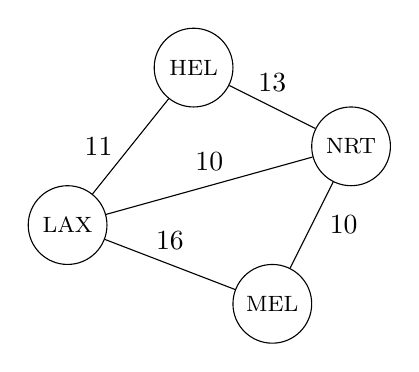
\begin{tikzpicture}[scale=2, every node/.style={draw, circle, minimum size=1cm}]
    % Nodes
    \node (HEL) at (0, .5) {\footnotesize HEL};
    \node (NRT) at (1, 0) {\footnotesize NRT};
    \node (MEL) at (.5, -1) {\footnotesize MEL};
    \node (LAX) at (-.8, -.5) {\footnotesize LAX};
    
    % Edges
    \draw (HEL) -- (NRT) node[midway, above=-2mm, draw=none, fill=none] {13};
    \draw (HEL) -- (LAX) node[midway, left=-1mm, draw=none, fill=none] {11};
    \draw (MEL) -- (LAX) node[midway, above=-2mm, draw=none, fill=none] {16};
    \draw (LAX) -- (NRT) node[midway, above=-2mm, draw=none, fill=none] {10};
    \draw (MEL) -- (NRT) node[midway, right=-1mm, draw=none, fill=none] {10};

\end{tikzpicture}
\caption{Flight network as a $K$-interpretation. \label{fig:air}}
\end{figure}

\begin{example}
    Suppose $A$ consists of the airport codes HEL, NRT, LAX, MEL, and $\tau$ of one edge relation $E$. Consider the tropical semiring $\mathbb{T}=(\mathbb{R}\cup\{\infty\}, \min, +, \infty, 0)$.
    An example $\mathbb{T}$-interpretation $\pi\colon Lit_{A,\tau}\to \mathbb{T}$ is obtained by assigning $E(x,y)$, for each pair of airports $x$ and $y$, a number representing the duration of a direct flight between them, as in \Cref{fig:air};
    if no direct flight exists between two airports $x$ and $y$, $E(x,y)$ is assigned $\infty$. Furthermore each negated fact $\neg E(x,y)$ can be assigned a number so that $\pi$ is model-defining.
    %
    Then, we can express in $\FO[<]$ that the duration of a direct flight between any two airports $x$ and $y$ is shorter than the sum of durations for flights from $x$ to  $z$ and $z$ to $y$, for any airport $z$:
    \[
    \phi \coloneqq \forall xyz( R(x,z) \land R(z,y) < R(x,y)).
    \]
    Clearly, $\evaluate{\phi}{\pi}=0$, that is, $\phi$ evaluates to the identity element of multiplication under $\pi$.
\end{example}


Let $\mathcal{A}$ be a structure of vocabulary $\tau$, and let $\mathbb{B}$ be the Boolean semiring. The canonical truth interpretation $\pi_{\mathcal{A}}$, is the $\mathbb{B}$-interpretation $\pi\colon\lit_{A,\tau}\to \mathbb{B}$ defined for each $R(\bar{a})$ and $\neg R(\bar{a})$ as follows
 \[
    \pi(R(\bar{a}))= 
    \begin{cases}
        1 \qquad\text{ if } \bar{a}\in R^{\mathcal{A}}\\
      0 \qquad\text{ if } \bar{a}\not\in R^{\mathcal{A}},
    \end{cases}
    \]
and $\pi(\neg R(\bar{a}))=1-\pi(R(\bar{a}))$.


The following proposition shows that for $\FO$-formulas, the canonical truth interpretation $\pi_{\mathcal{A}}$ under an assignment $s$ corresponds to the usual first-order formula evaluation under $s$ in the structure $\mathcal{A}$. 
It can be proven by induction on $\alpha$.
\begin{proposition}[\cite{gradel17semiringprovenancefirstordermodel}]
   Let $\alpha$ be an $\FO$-formula, and $\mathcal{A}$ a structure. Then  $\evaluate{\alpha}{\pi_{\mathcal{A}},s}=1$ if and only if $\mathcal{A}\models_s\alpha$.
\end{proposition}
% \begin{proof}
%     By easy induction on $\alpha$.
% \end{proof}
Let $\xi_K\colon K\to\mathbb{B}$ be the characteristic mapping such that $\xi_K(a)=0$ if $a$ is the zero element of $K$ and $\xi_K(a)=1$ otherwise. 
\begin{proposition}[\cite{BarlagHKPV23}]\label{equivprop}
    Let $K$ be a positive semiring, and $\pi\colon \lit_{A,\tau}\to K$ an interpretation. Then for all $\alpha\in\FO$, $\evaluate{\alpha}{\pi}=0$ if and only if $\evaluate{\alpha}{\xi_K\circ\pi}=0$.
\end{proposition}

%We say that a $K$-structure $\mathcal{A}$ of a vocabulary $\tau$ is \textit{model-defining}, if for all $R\in\tau$, we have $f_{R}^{\mathcal{A}}(\bar{a})=0$ iff $f_{\neg R}^{\mathcal{A}}(\bar{a})\neq 0$.

%Model-defining $K$-interpretation, add definition. 
%Maybe allow negation more generally? Otherwise, don't include the following proposition.

%\begin{proposition}
 %   Let $K$ be a positive (ordered) semiring, and $\pi$ a model-defining $K$-interpretation. For a $FO_K(=,\neq,\leq,\not\leq)$-formula $\phi$, $\pi(\phi)=0$ iff  $\pi(\neg\phi)\neq 0$.
%\end{proposition}

Sentences $\phi$ and $\psi$ of $\FO(O)$ are $K$-equivalent, written as $\phi\equiv_K \psi$, if $\evaluate{\phi}{\pi}=\evaluate{\psi}{\pi}$ for all 
%model-defining
$K$-interpretations. For logics $\mathcal{L}$ and $\mathcal{L}'$, we write $\mathcal{L}\leqq_K\mathcal{L}'$ if for each sentence $\phi$ from $\mathcal{L}$ there is a sentence $\psi$ from  $\mathcal{L}'$ such that $\phi\equiv_K \psi$. If $\mathcal{L}\leqq_K\mathcal{L}'$ and $\mathcal{L}'\leqq_K\mathcal{L}$, we write $\mathcal{L}\equiv_K\mathcal{L}'$, and say that $\mathcal{L}$ and $\mathcal{L}'$ are \textit{equally expressive under} K.

In case of the Boolean semiring $\mathbb{B}$ (with $0<1$), having access to formula (in)equality does not increase expressivity in the sense of the following proposition.
\begin{proposition}[\cite{BarlagHKPV23}]
$\FO\equiv_{\mathbb{B}}\FO(=,\neq,\leq,\not\leq)$
\end{proposition}
\begin{proof}
    Follows by simple induction from the fact that we have the following ${\mathbb{B}}$-equivalences  $\phi\leq \psi\equiv_{\mathbb{B}} \nnf(\neg\phi)\lor\psi$,  $\phi\not\leq \psi\equiv_{\mathbb{B}} \phi\wedge \nnf(\neg\psi)$, $\phi= \psi\equiv_{\mathbb{B}} (\phi\wedge\psi)\lor(\nnf(\neg\phi)\wedge \nnf(\neg\psi))$, and $\phi\neq \psi\equiv_{\mathbb{B}} (\nnf(\neg\phi)\wedge \psi)\lor(\phi\wedge \nnf(\neg\psi))$, where we use the notation $\nnf(\neg\alpha)$, $\alpha\in\FO$ for the formula obtained from $\neg\alpha$ by pushing the negation in front of the atomic formulas.
\end{proof}
The following example shows that the above proposition does not hold for all $K$.
\begin{example}
Let $\mathbb{N}=(\mathbb{N},+,\cdot,0,1)$ be the semiring of natural numbers. Then
    \[
\FO\not\equiv_{\mathbb{N}}\FO(=,\neq,\leq,\not\leq).
    \]
     Define $\phi=\forall x P(x)=\forall x Q(x)$. We show that $\phi$ cannot be translated to $\FO$. Suppose for a contradiction that $\alpha_{\phi}\in\FO$ is such that $\alpha_{\phi}\equiv_{\mathbb{N}}\phi$.
     Let $A=\{1,\dots, n\}$, $\tau=\{P,Q\}$, $\ar(P)=\ar(Q)=1$, and the interpretations $\pi\colon\lit_{A,\tau}\to \mathbb{N}$ and $\pi'\colon\lit_{A,\tau}\to \mathbb{N}$ be such that, for all $i\in A$,
     \begin{itemize}
         \item 
     $\pi(P(i))=1$, $\pi(\neg P(i))=0$, $\pi(Q(i))=1$, $\pi(\neg Q(i))=0$; and
     \item $\pi'(P(i))=1$, $\pi'(\neg P(i))=0$, $\pi'(Q(i))=2$, $\pi'(\neg Q(i))=0$.
     \end{itemize}
       Then $\evaluate{\phi}{\pi}=1$, because $\evaluate{\forall x P(x)}{\pi}=1$ and $\evaluate{\forall x Q(x)}{\pi}=1$. On the other hand, $\evaluate{\phi}{\pi'}=0$, because $\evaluate{\forall x P(x)}{\pi'}=1$ and $\evaluate{\forall x Q(x)}{\pi'}=2^n$. 
     
     Now $\evaluate{\alpha_{\phi}}{\pi}=\evaluate{\phi}{\pi}=1$ and $\evaluate{\alpha_{\phi}}{\pi'}=\evaluate{\phi}{\pi'}=0$, so by Proposition~\ref{equivprop}, $\evaluate{\alpha_{\phi}}{\xi_{\mathbb{N}}\circ\pi}\neq 0$ and $\evaluate{\alpha_{\phi}}{\xi_{\mathbb{N}}\circ\pi'}= 0$. But since $\xi_{\mathbb{N}}\circ\pi=\xi_{\mathbb{N}}\circ\pi'$, this is impossible.

     Note that similar arguments show that the sentences $\forall x P(x)\neq\forall x Q(x)$, $\forall x Q(x)\leq\forall x P(x)$, and $\forall x Q(x)\not\leq\forall x P(x)$ cannot be translated to $\FO$ either. 
\end{example}
%\minna{Earlier comment: Maybe add an example that shows that this is not the case for all $K$? Now: Added the above example.}
%\teemu{This (above) would probably be good for motivation, unless some example of this sort
%appears in some other paper?}

In order to compare this logic to the machine models we introduced, we need to identify it with a fitting set of functions.
For any $O \subseteq \{=, \neq, \leq, \not\leq\}$, any $\FO(O)$ sentence can essentially be seen as a function from the set of $K$-interpretations to $K$.
To make this fit in with our machine models, we define an encoding for $K$-interpretations, so that the function defined by an $\FO(O)$ sentence can be seen as function from $K^*$ to $K$.

%\nicolas{Does $A$ need to be ordered? What we really need is $\lit_{A, \tau}$ to be ordered.}
%\juha{The order on A allows us to order the literals using the induced lexicographic order.}
%\timon{only, if $\tau$ is also ordered}
\begin{definition}
    % \timon{need an ordering on $\lit_{A, \sigma}$ for this}
    Let $A$ be a strictly ordered set, let $\tau$ be a relational signature, let $\lit_{A, \tau} = \{\ell_1, \dots, \ell_n\}$, let $K$ be a 
    positive 
    semiring and let $\pi \colon \lit_{A, \tau} \to K$ be a $K$-interpretation.
    Then we define $\enc(\pi)$ to be the concatenation of the values assigned to each literal by $\pi$, i.e., 
    \[
        \enc(\pi) \coloneqq (\pi(\ell_1), \dots, \pi(\ell_n)) \in K^n.
    \]
    For technical reasons, we encode literals of relation symbols $R$ of arity $0$ as if they had arity $1$, i.e, as $\lvert A \rvert$ copies of $\pi(R())$.\label{def:enc}
\end{definition}

Of particular interest is that we can determine $\lvert A \rvert$ from $\lvert \enc(\pi) \rvert$.
% For this reason we make a minor technical change to the previous definition:
% for any $R \in \tau$ such that $\ar(R) = 0$, we regardless encode $R$ as $\lvert A \rvert$ copies of $\pi(R())$.
With this minor technical change at hand, we can now compute $\lvert A \rvert$ from $\lvert \enc(\pi) \rvert$ and $\tau$.

\begin{lemma}\label{lem:decode_A_size}
    Let $A$ be a strictly ordered set, let $\tau$ be a relational vocabulary, let $K$ be a semiring and $\pi \colon \lit_{A, \tau} \to K$ be a $K$-interpretation.
    We can compute $\lvert A \rvert$ when given $\lvert \enc(\pi) \rvert$ in logarithmic time on a $\BSSK$ machine.
\end{lemma}
\begin{proof}
We can use, e.g., binary search to find the solution for $\lvert A \rvert$ in
\[
    \lvert \enc(\pi) \rvert = \sum_{R \in \tau} \lvert A \rvert^{\max(\ar(R), 1)} \cdot 2
\]
in logarithmic time.
\end{proof}

To characterize circuit classes logically later on, we need to extend this logic by additional ``built-int'' $K$-relations that are not part of the $K$-interpretation. %and whose interpretation is determined by the size of the model.
To that end we will slightly extend the syntax of $\FO(O)$ to $\FO(O, F)$ for particular function families $F$.
We essentially want to allow additional $K$-relations that may depend on the size of $A$, but not on $A$ itself. 
We therefore treat ordered sets of the same cardinality as isomorphic to the first $\lvert A \rvert$ natural numbers and thus define the aforementioned function families accordingly.
The set $\arb$ is the set of all function families of the aforementioned kind.

\begin{definition}
Let $K$ be a semiring. 
Then 
\[
    \arb \coloneqq \bigcup_{k \in \N} \{(f_n)_{n \in \N} \mid \text{$f_n \colon \{1, \dots, n\}^k \to K$ for all $n \in \N$}\}.
\]
\end{definition}
% \juha{in the classical case we need built-in relations of arbitrary arities. Should this be incorporated also to the above definition?}
We also need to extend the notion of a signature to allow to differentiate between built-in $K$-relations and those given by the input $K$-interpretation.

\begin{definition}
    Let $O \subseteq \{=, \neq, \leq, \not\leq\}$, let $\tau$ and $\sigma$ be relational vocabularies and let $K$ be a positive semiring.
    Then for any set of function families $F \subseteq \arbF$ we define the syntax of $\FO(O, F)$ formulae over a signature $(\tau, \sigma)$ by extending the Backus-Naur-form for $\FO(O)$ formulae by the rule
    \[
        \alpha \Coloneqq P(\ol{x}) \mid \neg P(\ol{x}),
    \]
    where $P \in \sigma$ and $\ol{x}$ is a tuple of variables such that $\lvert \ol{x} \rvert = \ar(P)$.
\end{definition}

Defining the semantics of $\FO(O, F)$ requires a bit of care.
%In the Boolean setting, extending first-order logic in this way would be done by requiring that given a $(\tau, \sigma)$-sentence, there exists an interpretation for the symbols in $\sigma$ as built-in relations such that the given sentence is satisfied by a given $K$-interpretation. 
%Since the values we are dealing with are no longer merely Boolean, this approach does not work here.
We give each function family in $F$ a \emph{fixed} symbol, such that each symbol $P$ in $\sigma$ is interpreted as its predefined counterpart in $F$. Note also that, unlike in the classical setting, negative occurrences of each $P\in \sigma$ need a separate interpretation in $F$. %\juha{I think fixing a interpretation for each built-in relation symbol is a standard practice. With Arb also the "existential" interpretation works. }

% \begin{definition}
% \timon{version 1 of $\FO(O, F)$ semantics definition}
%     % Let $O \subseteq \{=, \neq, \leq, \not\leq\}$, let $F \subseteq \arbF$ be a family of functions, let $\tau$ be a finite, relational vocabulary, let $\sigma$ be a vocabulary such that $\lvert F \rvert = 2 \cdot \lvert \sigma \rvert$ and let $I_{F, \sigma}$ be an interpretation which bijects $F$ and $\sigma \cup \left\{\neg P \mid P \in \sigma \right\}$.

%     Let $O \subseteq \{=, \neq, \leq, \not\leq\}$, let $K$ be a positive semiring let $F \subseteq \arbF$ be a family of functions, let $\tau$ and $\sigma$ be finite, relational vocabularies, such that $\lvert F \rvert \geq 2 \cdot \lvert \sigma \rvert$ and let $I_{F, \sigma}$ be an interpretation which is a total function from $\sigma \cup \left\{\neg P \mid P \in \sigma \right\}$ to $F$.\juha{I guess we could assume that P can be only used in positive contexts}

%     % let $\tau$ and $\sigma$ be finite, relational vocabularies, such that $\lvert F \rvert \geq 2 \cdot \lvert \sigma \rvert$ and let $(\rho_n)_{n \in \N}$ be a family of $K$-interpretations such that $\rho_n \colon \lit_{\{1, \dots, n\}, \sigma} \to K$ for all $n \in \N$.
    
%     Let furthermore $A$ be a strictly ordered set\juha{I guess we need a strict linear order} and $\pi \colon \lit_{A, \tau}$ be a $K$-interpretation and $s$ be an assignment.
%     Then the semantics of $\FO(O, F, I_{F, \sigma})$ extend the semantics for $\FO(O)$ by 
%     \[
%         \evaluate{P(\ol{x})}{\pi, s} = P^{I_{F, \sigma}}(r(s(\ol{x}))), \qquad \evaluate{\neg P(\ol{x})}{\pi, s} = (\neg P)^{I_{F, \sigma}}(r(s(\ol{x}))),
%     \]
%     where $P \in \sigma$, $P^{I_{F, \sigma}}$ and $(\neg P)^{I_{F, \sigma}}$ are the respective interpretations of $P$ and $\neg P$ according to $I_{F, \sigma}$, $\ol{x}$ is a tuple of variables such that $\lvert \ol{x} \rvert = \ar(P)$ and $r \colon A \to \{1, \dots, \lvert A \rvert\}$ is the \emph{ranking function} on $A$, which maps each element of $A$ to its position in the ordering on $A$.

%     For brevity, we generally omit the $I_{F, \sigma}$ in the notation and just write $\FO(O, F)$ instead of $\FO(O, F, I_{F, \sigma})$.
% \end{definition}

% \begin{definition}
% \timon{version 2 of $\FO(O, F)$ semantics definition}
%     % Let $O \subseteq \{=, \neq, \leq, \not\leq\}$, let $F \subseteq \arbF$ be a family of functions, let $\tau$ be a finite, relational vocabulary, let $\sigma$ be a vocabulary such that $\lvert F \rvert = 2 \cdot \lvert \sigma \rvert$ and let $I_{F, \sigma}$ be an interpretation which bijects $F$ and $\sigma \cup \left\{\neg P \mid P \in \sigma \right\}$.

%     % let $\tau$ and $\sigma$ be finite, relational vocabularies, such that $\lvert F \rvert \geq 2 \cdot \lvert \sigma \rvert$ and let $I_{F, \sigma}$ be an interpretation which is a total function from $\sigma \cup \left\{\neg P \mid P \in \sigma \right\}$ to $F$.

%     Let $O \subseteq \{=, \neq, \leq, \not\leq\}$, let $F \subseteq \arbF$ be a family of functions, let $\tau$ and $\sigma$ be finite, relational vocabularies, such that $\lvert F \rvert \geq 2 \cdot \lvert \sigma \rvert$ and let $(\rho_n)_{n \in \N}$ be a family of $K$-interpretations such that $\rho_n \colon \lit_{\{1, \dots, n\}, \sigma} \to K$ for all $n \in \N$.
    
%     Let furthermore $A$ be an ordered set, let $\pi \colon \lit_{A, \tau} \to K$ be a $K$-interpretation and $s$ be an assignment.
%     Then the semantics of $\FO(O, F, \rho)$ extend the semantics for $\FO(O)$ by 
%     \[
%         \evaluate{P(\ol{x})}{\pi, \rho, s} = \rho_{\lvert A \rvert}(P(r(s(\ol{x})))), \qquad \evaluate{\neg P(\ol{x})}{\pi, \rho, s} = \rho_{\lvert A \rvert}(\neg P(r(s(\ol{x}))))
%     \]
%     where $P \in \sigma$, $\ol{x}$ is a tuple of variables such that $\lvert \ol{x} \rvert = \ar(P)$ and $r \colon A \to \{1, \dots, \lvert A \rvert\}$ is the \emph{ranking} function on $A$, which maps each element of $A$ to its position in the ordering on $A$.

%     For brevity, we generally omit the $\rho$ in the notation and just write $\FO(O, F)$ instead of $\FO(O, F, \rho)$.
% \end{definition}
\begin{definition}
% \timon{version 2 of $\FO(O, F)$ semantics definition}
    % Let $O \subseteq \{=, \neq, \leq, \not\leq\}$, let $F \subseteq \arbF$ be a family of functions, let $\tau$ be a finite, relational vocabulary, let $\sigma$ be a vocabulary such that $\lvert F \rvert = 2 \cdot \lvert \sigma \rvert$ and let $I_{F, \sigma}$ be an interpretation which bijects $F$ and $\sigma \cup \left\{\neg P \mid P \in \sigma \right\}$.

    % let $\tau$ and $\sigma$ be finite, relational vocabularies, such that $\lvert F \rvert \geq 2 \cdot \lvert \sigma \rvert$ and let $I_{F, \sigma}$ be an interpretation which is a total function from $\sigma \cup \left\{\neg P \mid P \in \sigma \right\}$ to $F$.

    Let $O \subseteq \{=, \neq, \leq, \not\leq\}$, let $K$ be a positive semiring, let $F \subseteq \arbF$ be a family of functions, let $\tau$ and $\sigma$ be finite, relational vocabularies, such that $\lvert F \rvert \geq 2 \cdot \lvert \sigma \rvert$ and let $(\rho_n)_{n \in \N}$ be a family of $K$-interpretations such that for each $P \in \sigma$ there exist families $(f_n)_{n \in \N}$ and $(f'_n)_{n \in \N}$ in $F$, such that $\rho_n(P(\ol{a})) = f_n(\ol{a})$ and $\rho_n(\neg P(\ol{a})) = f'_n(\ol{a})$ for all $\ol{a} \in \{1, \dots, n\}^{\ar(P)}$.
    
    Let furthermore $A$ be a strictly ordered set, let $\pi \colon \lit_{A, \tau} \to K$ be a $K$-interpretation and $s$ be an assignment.
    Then the semantics of $\FO(O, F, \rho)$ extend the semantics for $\FO(O)$ by 
    \[
        \evaluate{P(\ol{x})}{\pi, \rho, s} = \rho_{\lvert A \rvert}(P(r(s(\ol{x})))), \qquad \evaluate{\neg P(\ol{x})}{\pi, \rho, s} = \rho_{\lvert A \rvert}(\neg P(r(s(\ol{x})))),
    \]
    % \timonS{In all other cases, the $\rho$ in $\evaluate{.}{\pi, \rho, s}$ does nothing.}
    where $P \in \sigma$, $\ol{x}$ is a tuple of variables such that $\lvert \ol{x} \rvert = \ar(P)$ and $r \colon A \to \{1, \dots, \lvert A \rvert\}$ is the \emph{ranking function} on $A$, which maps each element of $A$ to its position in the ordering on $A$.

    In the cases where $\rho$ is not relevant for the semantics, it is omitted, to stay consistent with the notation in Definition~\ref{interpretation}.
    % For brevity, whenever there is no risk of ambiguity, we omit the $\rho$ in the notation and just write $\FO(O, F)$ instead of $\FO(O, F, \rho)$.
\end{definition}

With this definition at hand, we can finally define the set of functions definable by $\FO(O, F)$ sentences.
Note that we omit $O$ (resp. $F$), if it is empty.

\begin{definition}
Let $O \subseteq \{=, \neq, \leq, \not\leq\}$ and let $F \subseteq \arbF$.
For a semiring $K$ and an $\FO(O, F)$ sentence $\varphi$, we define the function problem $\FOK(O, F) \EVAL_\varphi \colon K^* \to K$ as follows:
\end{definition}
\funcproblemdef{$\FOK(O,F, \rho)\EVAL_\varphi$}{an encoded $K$-interpretation $\enc(\pi)$}{$\evaluate{\varphi}{\pi, \rho}$}
% \timon{This requires that $A$ is ordered by a strict, total order, so that the encoding is unambiguous.}
% \timon{Also technically, the Output should be $\evaluate{\varphi}{\pi, \rho}$}

To denote the set of all these function problems, we introduce the following notation.

\begin{definition}
Let $O \subseteq \{=, \neq, \leq, \not\leq\}$, let $K$ be a positive semiring, and $F \subseteq \arbF$. 
Then
\[
\begin{array}{r@{\,}l}
     \FOK &\coloneqq \{\,\FOK\EVAL_\varphi\mid \varphi \in \FO\,\}\\
        \FOK(O) &\coloneqq \{\,\FOK(O)\EVAL_\varphi\mid \varphi \in \FO(O)\,\}\\
        \FOK(O, F) &\coloneqq \{\,\FOK(O, F)\EVAL_\varphi\mid \exists \rho:~ \varphi \in \FO(O, F, \rho)\,\}
\end{array}
\]
\end{definition}
% \arne[inline]{I did not get what $F$ really is and how $\FOK(O, F)\EVAL_\varphi$ is defined. Can you explain please? What does ``$f_n\colon\{1,\dots,n\}$ for all $n$'' mean?}
% \timon{The $F$ will be the built-in functions. 
% The nonuniform circuit result will have the form FO[Arb] = $\ACO$ as in the classical case, and the $F$ is where we stick in the Arb.
% The ``$f_n\colon\{1,\dots,n\}$ for all $n$'' was missing ``$\to K$''. 
% These are the function families we add, which can depend only on the size of the input $A$, so we treat all sets of the same size as isomorphic.
% }
% \vivian{maybe write $\FOK\EVAL$ on the left to make clear, those are the eval classes?}
% \timon{We could do that. 
% I was thinking of using the notation $\FOK\EVAL$ to denote functions of the form basically $(\pi, \varphi) \to K$.
% Currently $\FOK$ is a set of functions of the form $\pi \to K$ and we would still need another name for sets of functions $(\pi, \varphi, s) \to K$, because that is basically what the function version of the model checking problem will be.
% }

% \noindent\fbox{\parbox{\textwidth}{
% \timon{still need the following:}
% \begin{itemize}
%     \item def FO(Arb)
%     \item[$\to$] probably generalize FO[=] def
%     \item somehow specify what happens if the input for $\FOK\EVAL_\varphi$ is no encoding of a valid $K$-interpretation for $\varphi$
%     \item[$\to$] probably need to define signature of a formula and argue, when an element of $K^*$ is a valid encoding of a $K$-interpretation for a formula
% \end{itemize}
% }}

In the upcoming sections, we establish several connections between the previously introduced models of computation and logic.
It is noteworthy that our results generalize beyond model-defining $K$-interpretations, as defined on page~\pageref{par:model_defining}.

\section{The Complexity of Model Checking for \texorpdfstring{$\FOK$}{FOK}}\label{results}

We assume basic familiarity with computational complexity theory~\cite{DBLP:books/daglib/0018514}. 
In the following, we define the model checking problem. 
\decproblemdef{$\FOKMC{}$, $O\subseteq\{=,\neq,\leq,\not\leq\}$, semiring $K$}{an $\FOK(O)$ formula $\varphi$, a $K$ interpretation $\pi$, an assignment $s$, a set $A$}{$\evaluate{\varphi}{\pi,s}\neq0$}
%\minna{If we consider the version where we just check whether $\evaluate{\varphi}{\pi,s}\neq0$, should we have $\FO(O)$ for some $O$ s.t. $\emptyset\neq O\subseteq\{=,\neq,\leq,\not\leq\}$ instead of just $\FO$? See Prop~\ref{equivprop}. Or maybe I am misunderstanding something? Otherwise, it seems to me that by Prop~\ref{equivprop}, it is enough to check this for $\mathbb{B}$ by using $\xi_K\circ\pi$?}
For instance, if we are interested in the data complexity of the problem, then we write, e.g., $\FOKMC{\varphi}$ to emphasise on the fact that $\varphi$ is fixed. 

Regarding input values, we assume for $\varphi$, $s$, and $A$ standard polynomial-time computable encodings, e.g., binary encoding. 
For $\pi$, we use $\enc(\pi)$ specified in Def.~\ref{def:enc}.

%\subsection{BSS machines}
%\nicolas{Classical Result: Model checking can be done in time $O(|\varphi| \cdot |\mathfrak{A}|^k)$ with $k$ the maximum number of free variables in a subformula of $\varphi$. \cite[Prop.~6.6]{DBLP:books/sp/Libkin04}}
\begin{theorem}
    Fix a positive commutative semiring $K$. 
    Given an $\FOK$ formula $\varphi$, a $K$ interpretation $\pi$, an assignment $s$, and a set $A$. 
    The value $\evaluate{\varphi}{\pi,s}$ can be computed in time $\bO(n^2 \cdot |\varphi| \cdot |A|^{|\varphi|})$ and space in $\bO(\mathrm{poly}(n))$, with $n = |\varphi|+|\pi|+|s|+|A|$ the sum of the encoding lengths.
\end{theorem}
\begin{algorithm}[t]
    \DontPrintSemicolon
    \SetKwInOut{Data}{Data}
    \SetKwProg{Proc}{Procedure}{}{}
    \KwData{set $A$, $K$-interpretation $\pi$}
    \Proc{\procEval(formula $\varphi$, assignment $s$)}{
    \Switch(\tcp*[f]{time complexity}){$\varphi$}{
        \lCase(\tcp*[f]{$\bO(n)$}){$x = y$}{\Return 1 iff $s(x) = s(y)$}
        \lCase(\tcp*[f]{$\bO(n)$}){$x \neq y$}{\Return 1 iff $s(x) \neq s(y)$}
        \lCase(\tcp*[f]{$\bO(n^2)$}){$ R(\bar x)$}{\Return $\pi(R(s(\bar x)))$}
        \lCase(\tcp*[f]{$\bO(n^2)$}){$\lnot R(\bar x)$}{\Return $\pi(\lnot R(s(\bar x)))$}
        \lCase(\tcp*[f]{$\bO(n) + t(\psi) + t(\theta)$}){$\psi \land \theta$}{\Return $\procEval(\psi, s) \cdot \procEval(\theta, s)$}
        \lCase(\tcp*[f]{$\bO(n) + t(\psi) + t(\theta)$}){$\psi \lor \theta$}{\Return $\procEval(\psi, s) + \procEval(\theta, s)$}
        \lCase(\tcp*[f]{$\bO(n) + t(\psi) + t(\theta)$}){$\psi \star \theta$}{\Return 1 iff $\procEval(\psi, s) \star \procEval(\theta, s)$}
        \lCase(\tcp*[f]{$|A| \cdot \bO(n)\cdot t(\psi)$}){$\exists x \psi$}{\Return $\sum_{a \in A}\procEval(\psi, s[a/x])$}
        \lCase(\tcp*[f]{$|A| \cdot \bO(n)\cdot t(\psi)$}){$\forall x \psi$}{\Return $\prod_{a \in A}\procEval(\psi, s[a/x])$} 
    }
    }
\caption{Evaluation of $\evaluate{\varphi}{\pi, s}$, where $\star\in O\subseteq\{=,\neq,\leq,\not\leq\}$ }
\label{alg:evaluation of varphi}
\end{algorithm}
\begin{proof}
The procedure $\procEval$ in Algorithm~\ref{alg:evaluation of varphi} is a recursive algorithm that runs on a $K$-TM to solve the model checking problem. 
Set $A$ and $\pi$ are used as ``global variables'' as they are never modified in the recursive steps. 
They are accessible by every recursive algorithmic call. 
The correctness follows inductively by semantics (Def.~\ref{interpretation}). 

Now let $n$ be the input length, i.e., $n=|\varphi|+|\pi|+|s|+|A|$. 
To measure the space used by the machine, we need to prove an upper bound on the recursion depth and the space used in a recursive step. 
For every conjunction and disjunction there are two recursive steps. 
For every quantifier there are $|A|$-many recursive steps. 
So altogether, we can bound the number of recursive steps as follows for a given formula $\varphi$:
\[
    (2\cdot(\#_\land(\varphi)+\#_\lor(\varphi))+1) \cdot |A|^{(\#_\exists(\varphi)+\#_\forall(\varphi))} \in \bO(|\varphi|\cdot|A|^{|\varphi|}),
\]
where $\#_O(\varphi)$, for $O\in\{\land,\lor,\exists,\forall\}$, is the number of occurrences of $O$ in $\varphi$. 
Now, we turn towards the space and time bound of a single recursive step. 
We do a case distinction according to the \textbf{switch}-expression in the algorithm.
\begin{description}
    \item[$x=y$ / $x\neq y$:] Use separate registers in $R$ to copy and check if such an expression is true. This needs constant space and linear time in $n$.
    \item[$R(\bar x)$ / $\lnot R(\bar x)$:] Copy the values of $s(\bar x)$ to the end of the tape and return the specified value according to $\pi$. For that purpose, we need additional markings to ``remember'' which positions have been compared. Altogether this can be done in quadratic time in $n$ and linear space in $n$.
    \item[$\wedge$ / $\vee$:] Here, we need to copy the respective parts from the input yielding $\bO(n)$ time and space.
    \item[$\star$:] Analogously as for the previous case.
    \item[$\exists$ / $\forall$:] %Recall that $c=|A|$. 
    Again, we essentially need to copy parts from the input and patch the assignment. 
    Regarding the $A$-values we need to iterate through this part of the input yielding $\bO(n)$ time and space.
\end{description}
We see that the space of each step is bounded by $\bO(n)$. 
Regarding time complexity, 
the time needed at each step is in $\bO(n^2)$ and the number of recursive steps was bounded by $\bO(|\varphi| \cdot |A|^{\varphi})$
% the recursion depth was linear in $|\varphi|$ and the branching degree was bounded by $|A|$ 
yielding a time bound of $\bO(n^2 \cdot |\varphi| \cdot |A|^{|\varphi|})$.
\end{proof}
\begin{corollary}
Let $O \subseteq \{=, \neq, \leq, \not\leq\}$ and $F \subseteq \arbF$.
    Every $f\in\FOK(O,F)$ can be computed in polynomial space.
\end{corollary}
% \juha{arities of build in functions can be more than 1 in the above corollary also?}
% \arne[inline]{The next result should be in constant time even as $A$ and $|\varphi|$ are then constants?}
% \nicolas{the previous result should be time $O(n \cdot |A|^{|\varphi|})$?!}
The following two corollaries are obtained via utilisation of Algorithm~\ref{alg:evaluation of varphi} and merely checking whether the computed value of $\evaluate{\varphi}{\pi,s}$ is not $0$.
\begin{corollary}
    $\FOKMC{\varphi} \in \PK$ for every $O\subseteq\{=,\neq,\leq,\not\leq\}$.
\end{corollary}
% \begin{proof}
%     todo
% \end{proof}

\begin{corollary}
    $\FOKMC{} \in \PSPACEK$ for every $O\subseteq\{=,\neq,\leq,\not\leq\}$.
\end{corollary}
% \begin{proof}    
% \end{proof}


\section{A Circuit Characterisation of \texorpdfstring{$\FOK$}{FOK}}\label{circ}

The following is an adaptation of a result in the Boolean setting, first established by Immerman~\cite{DBLP:journals/siamcomp/Immerman87}.
It made rigorous intuition that first-order logic and constant-depth circuits more or less do the same thing.
More recently, this result has been generalized to metafinite logics over the reals~\cite{10.1093/logcom/exae051} and more general integral domains~\cite{BCG24}.
We establish a similar result, moving from integral domains to positive, commutative semirings and replacing logics over metafinite structures with a logic that is evaluated directly in the semiring.

\begin{theorem}\label{thm:fo_aco}
Let $O \subseteq \{=, \neq, \leq, \not\leq\}$ and let $K$ be a positive, commutative semiring. 
Then for $K$-interpretations $\pi \colon \lit_{\tau, A} \to K$, where $A$ is strictly ordered: $\FOK(O, \arb) = \FACO[O]$.
\end{theorem}

\begin{proof}
    This proof follows the same general pattern as a similar result about circuits over the reals and first-order logic over metafinite $\R$-structures \cite[Theorem~30]{10.1093/logcom/exae051}.
    
    The basic idea is for the direction $\FOK(O, \arb) \subseteq \FACO[O]$ to mimic the behaviour of quantifiers and logical connectives by means of the arithmetic gate types. 
    E.g., existential quantification can be simulated by an unbounded addition and a disjunction can be modeled by a multiplication gate.
    
    For the converse direction, we define a sentence that essentially describes the way a circuit is evaluated, using the additional built-in relations to describe the structure of the circuit.

    The full proof can be found in Appendix~\ref{proof:thm_fo_aco}.
\end{proof}


% \section{Comparing with Weights}

% Something about weighted TMs vs BSS$_K$ and something about weighted FO vs $FO_K$
% \vivian{maybe not needed as its own section, depends on our results}

\section{Conclusion}
% Extending the circuit result to uniform circuit and larger circuit classes. 
% Continue in the BSS setting to e.g. generalize Grädel and Meer's real version of Fagin's theorem~\cite{DBLP:conf/stoc/GradelM95} to semirings.

In this paper, we introduced several models of computation to analyze the complexity of problems with respect to semirings.
In particular, we adapted BSS-machines and arithmetic circuits for semirings to generalize previously established models for computation with fields or rings.
We then characterized the complexity of the model checking and evaluation problem of first-order logic with semiring semantics using these models.

The work in establishing a complexity theory started here gives rise to an abundance of further research directions.

Continuing from the model checking question, other possible connections between semiring logics and sequential computation merit investigation. 
In particular, the well-known theorem by Fagin, establishing a connection between second-order logic and NP~\cite{fagin1974generalized}, which has been adapted to BSS machines and logics over the real numbers by Grädel and Meer~\cite{DBLP:conf/stoc/GradelM95}, warrants analysis with respect to semirings.

%Another avenue of further research is the examination of logics with the recently established semiring team semantics~\cite{BarlagHKPV23} in terms of computational complexity over semirings.
% \juha{maybe not mention team semantics here?}
Furthermore, there is much work to be done with regard to arithmetic circuits over semirings. 
The result shown in this paper only pertains to so-called \emph{non-uniform} circuit families, meaning circuit families, where there is no restriction on how computationally difficult it is to obtain any individual circuit.
In general, this can lead to problems solvable by such circuit families, that are not computable with regard to BSS machines.
In order to view a circuit family as an algorithm, a restriction on how hard it is to obtain any given circuit is required.
Given the constructive nature of our proof, there is no doubt that it can be made uniform.
The exact nature of that uniformity still needs to be examined, however.
Additionally, larger circuit classes than $\FACO$ could be characterized, following, e.g., the characterization to the entire $\mathrm{AC}$ and $\mathrm{NC}$ hierarchies over the reals~\cite{BCG24}.

% \timon{mention $K$-TMs? Explicit questions w.r.t. $K$-team semantics?}

\bibliography{ref_url,references}

\newpage
\appendix
\section{Appendix} \label{appendix}
\begin{figure}[!h] % !h neccessar, otherwise appendix B starts immediately
    \centering
    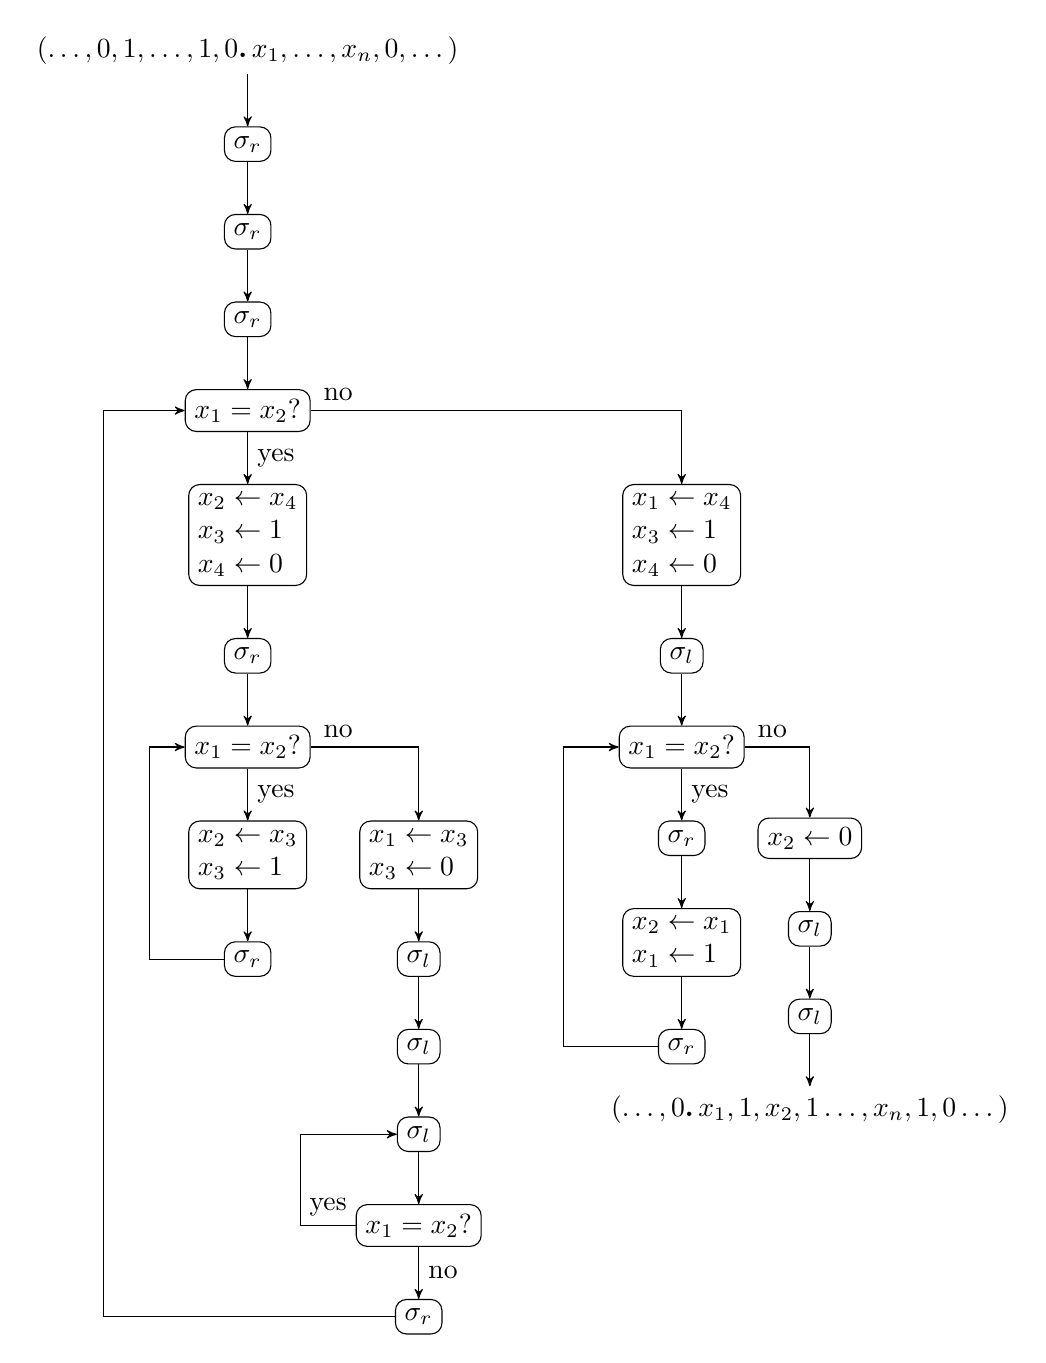
\begin{tikzpicture}[
        bssnode/.style = {draw, rounded corners},
        node distance=.66
        ]
        \node (0) {$(\dots, 0, 1, \dots, 1, 0\textbf{.}\, x_1, \dots, x_n, 0, \dots)$};
        \node[bssnode, below = of 0] (1) {$\sigma_r$};
        \node[bssnode, below = of 1] (2) {$\sigma_r$};
        \node[bssnode, below = of 2] (3) {$\sigma_r$};
        \node[bssnode, below = of 3] (4) {$x_1 = x_2$?}; % x_2 is always 1 here  
        \node[bssnode, below = of 4, align=left] (5) {$x_2 \gets x_4$\\$x_3 \gets 1$\\$x_4 \gets 0$};
        \node[bssnode, below = of 5] (6) {$\sigma_r$};
        \node[bssnode, below = of 6] (7) {$x_1 = x_2$?}; % x_2 is always 1 here  
        \node[bssnode, below = of 7, align=left] (8) {$x_2 \gets x_3$\\$x_3 \gets 1$};
        \node[bssnode, below = of 8] (9) {$\sigma_r$};
        \node[bssnode, right = of 8, align=left] (10) {$x_1 \gets x_3$\\$x_3 \gets 0$};
        \node[bssnode, below = of 10] (12) {$\sigma_l$};
        \node[bssnode, below = of 12] (12 1) {$\sigma_l$};
        \node[bssnode, below = of 12 1] (12 2) {$\sigma_l$};
        \node[bssnode, below = of 12 2] (13) {$x_1 = x_2$?}; % x_1 = x_2 until x_1 = 1 and x_2 = 0
        \node[bssnode, below = of 13] (13 1) {$\sigma_r$};
        
        \node[bssnode, right = 4cm of 5, align=left] (14) {$x_1 \gets x_4$\\$x_3 \gets 1$\\$x_4 \gets 0$};
        
        \node[bssnode, below = of 14] (15) {$\sigma_l$};
        % \node[bssnode, below = of 15] (16) {$x_2 \gets 1$};
        \node[bssnode, below = of 15] (17) {$x_1 = x_2$?}; 
        \node[bssnode, below = of 17] (18) {$\sigma_r$};
        \node[bssnode, below = of 18, align=left] (19) {$x_2 \gets x_1$\\$x_1 \gets 1$};
        \node[bssnode, below = of 19] (20) {$\sigma_r$};
        
        \node[bssnode, right = of 18] (21) {$x_2 \gets 0$};
        \node[bssnode, below = of 21] (22) {$\sigma_l$};
        \node[bssnode, below = of 22] (23) {$\sigma_l$};
        \node[below = of 23] (24) {$(\dots, 0\textbf{.}\, x_1, 1, x_2, 1 \dots, x_n, 1, 0 \dots)$};
        
        \draw[-stealth'] (0) -- (1);
        \draw[-stealth'] (1) -- (2);
        \draw[-stealth'] (2) -- (3);
        \draw[-stealth'] (3) -- (4);
        \draw[-stealth'] (4) -- node[right]{yes} (5);
        \draw[-stealth'] (5) -- (6);
        \draw[-stealth'] (6) -- (7);
        \draw[-stealth'] (7) -- node[right]{yes} (8);
        \draw[-stealth'] (8) -- (9);
        \draw[-stealth'] (9) -- ++(-1.25,0) |- (7);
        \draw[-stealth'] (7) -- node[above]{no} ++(1.5,0) -| (10);
        \draw[-stealth'] (10) -- (12);
        \draw[-stealth'] (12) -- (12 1);
        \draw[-stealth'] (12 1) -- (12 2);
        \draw[-stealth'] (12 2) -- (13);
        \draw[-stealth'] (13) -- node[above]{yes} ++(-1.5,0) |- (12 2);
        \draw[-stealth'] (13) -- node[right]{no} (13 1);
        \draw[-stealth'] (13 1) -- ++ (-4,0) |- (4);
        \draw[-stealth'] (4) -- node[above]{no} ++(1.5,0) -| (14);
        \draw[-stealth'] (14) -- (15);
        \draw[-stealth'] (15) -- (17);
        % \draw[-stealth'] (16) -- (17);
        \draw[-stealth'] (17) -- node[right]{yes} (18);
        \draw[-stealth'] (17) -- node[above]{no} ++(1.5,0) -| (21);
        \draw[-stealth'] (18) -- (19);
        \draw[-stealth'] (19) -- (20);
        \draw[-stealth'] (20) -- ++(-1.5,0) |- (17);
        \draw[-stealth'] (21) -- (22);
        \draw[-stealth'] (22) -- (23);
        \draw[-stealth'] (23) -- (24);
    \end{tikzpicture}
    \caption{\texttt{Init} subroutine. 
    Converts an input of a BSS$_K$ machine into gap normal form. 
    The elements on the right of the dot are always $x_1, x_2, \dots$ during the computation. 
    And $\sigma_l$ (resp. $\sigma_r$) shift the \textbf{state space} to the left (right) with respect to the dot.    
    The intuition of the algorithm is to iteratively pair each $x$ value with a 1.
    Also the shift and compare nodes are placed in such a way that no comparison with the input is made.
    This avoids problems when the input has 0 or 1 values.
    }
    \label{fig:bss normal form machine}
\end{figure}
\begin{figure}
    \centering
    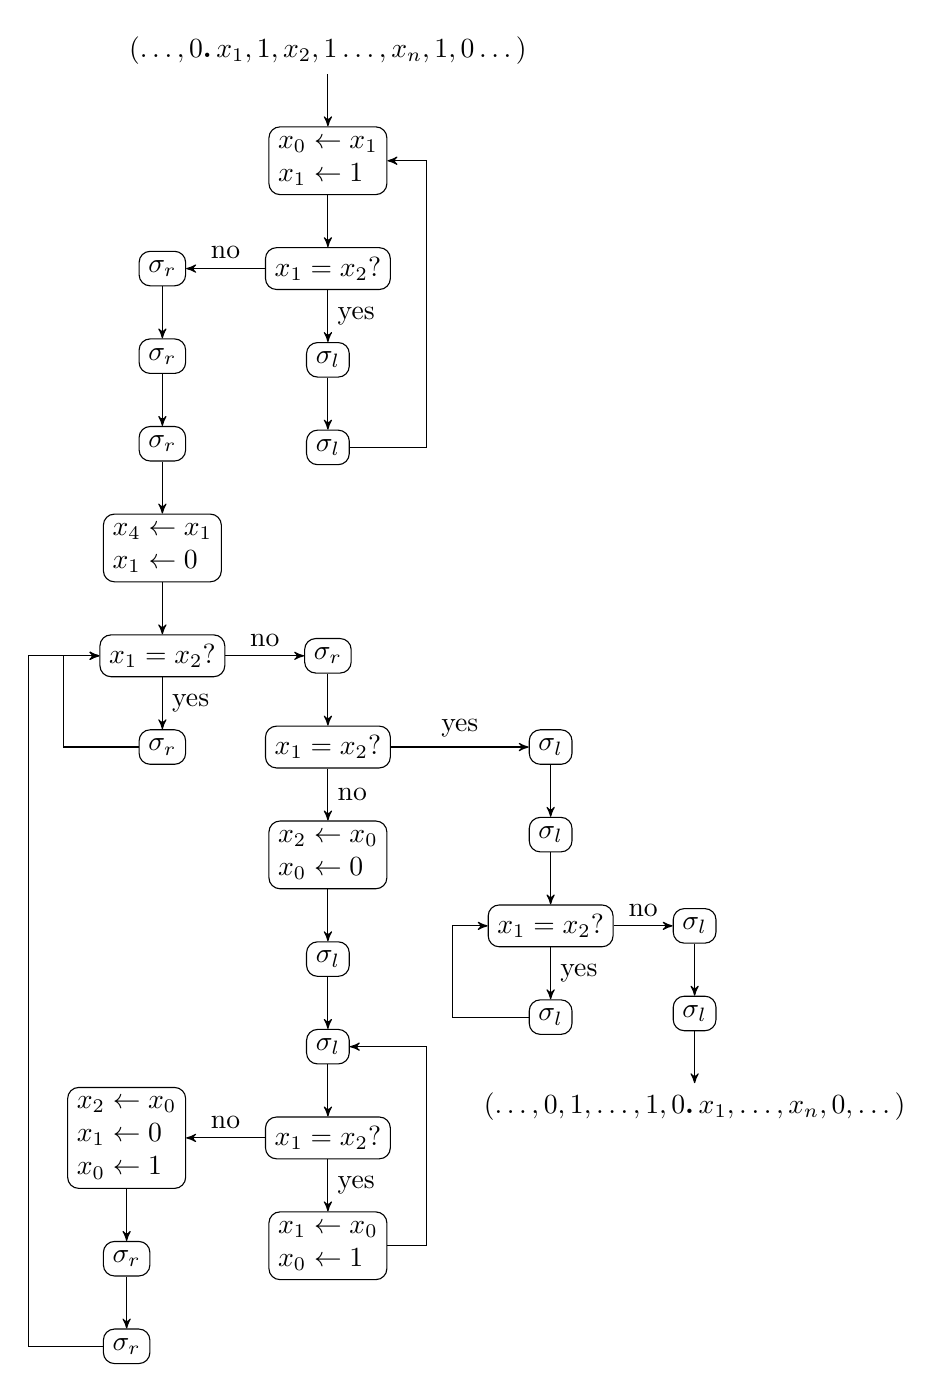
\begin{tikzpicture}[
        bssnode/.style = {draw, rounded corners},
        node distance=.66
        ]
        \node (0) {$(\dots, 0\textbf{.}\, x_1, 1, x_2, 1 \dots, x_n, 1, 0 \dots)$};
        \node[bssnode, below = of 0, align=left] (1) {$x_0 \gets x_1$\\$x_1 \gets 1$};
        \node[bssnode, below = of 1] (2) {$x_1 = x_2$?};
        \node[bssnode, below = of 2] (3) {$\sigma_l$};
        \node[bssnode, below = of 3] (4) {$\sigma_l$};
        \node[bssnode, left = 1cm of 2] (5) {$\sigma_r$};
        \node[bssnode, below = of 5] (6) {$\sigma_r$};
        \node[bssnode, below = of 6] (7) {$\sigma_r$};
        \node[bssnode, below = of 7, align=left] (8) {$x_4 \gets x_1$\\$x_1 \gets 0$};
        \node[bssnode, below = of 8] (9) {$x_1 = x_2$?};
        \node[bssnode, below = of 9] (10) {$\sigma_r$};
        \node[bssnode, right = 1cm of 9] (11) {$\sigma_r$};
        \node[bssnode, below = of 11] (12) {$x_1 = x_2$?};
        \node[bssnode, below = of 12, align=left] (13) {$x_2 \gets x_0$\\$x_0 \gets 0$};
        \node[bssnode, below = of 13] (14) {$\sigma_l$};        
        \node[bssnode, below = of 14] (15) {$\sigma_l$};
        \node[bssnode, below = of 15] (16) {$x_1 = x_2$?};
        \node[bssnode, below = of 16, align=left] (17) {$x_1 \gets x_0$\\$x_0 \gets 1$};
        \node[bssnode, left = 1cm of 16, align=left] (18) {$x_2 \gets x_0$\\$x_1 \gets 0$\\$x_0 \gets 1$};
        \node[bssnode, below = of 18] (19) {$\sigma_r$};
        \node[bssnode, below = of 19] (20) {$\sigma_r$};
        
        \node[bssnode, right = 1.75cm of 12] (21) {$\sigma_l$};
        \node[bssnode, below = of 21] (22) {$\sigma_l$};
        \node[bssnode, below = of 22] (23) {$x_1 = x_2$?};
        \node[bssnode, below = of 23] (24) {$\sigma_l$};
        \node[bssnode, right = 0.75cm of 23] (25) {$\sigma_l$};
        \node[bssnode, below = of 25] (26) {$\sigma_l$};        
        \node[below = of 26] (27) {$(\dots, 0, 1, \dots, 1, 0\textbf{.}\, x_1, \dots, x_n, 0, \dots)$};
        
        \draw[-stealth'] (0) -- (1);
        \draw[-stealth'] (1) -- (2);
        \draw[-stealth'] (2) -- node[right]{yes} (3);
        \draw[-stealth'] (3) -- (4);
        \draw[-stealth'] (4) -- ++(1.25,0) |- (1);
        \draw[-stealth'] (2) -- node[above]{no} (5);
        \draw[-stealth'] (5) -- (6);
        \draw[-stealth'] (6) -- (7);
        \draw[-stealth'] (7) -- (8);
        \draw[-stealth'] (8) -- (9);
        \draw[-stealth'] (9) -- node[above]{no} (11);
        \draw[-stealth'] (11) -- (12);
        \draw[-stealth'] (12) -- node[right]{no} (13);
        \draw[-stealth'] (9) -- node[right]{yes} (10);
        \draw[-stealth'] (10) -- ++(-1.25,0) |- (9);
        \draw[-stealth'] (13) -- (14);
        \draw[-stealth'] (14) -- (15);
        \draw[-stealth'] (15) -- (16);
        \draw[-stealth'] (16) -- node[right]{yes} (17);
        \draw[-stealth'] (16) -- node[above]{no} (18);
        \draw[-stealth'] (17) -- ++(1.25,0) |- (15);
        \draw[-stealth'] (18) -- (19);
        \draw[-stealth'] (19) -- (20);
        \draw[-stealth'] (20) -- ++(-1.25,0) |- (9);
        \draw[-stealth'] (12) -- node[above]{yes} (21);
        \draw[-stealth'] (21) -- (22);
        \draw[-stealth'] (22) -- (23);
        \draw[-stealth'] (23) -- node[right]{yes} (24);
        \draw[-stealth'] (24) -- ++(-1.25,0) |- (23);
        \draw[-stealth'] (23) -- node[above]{no} (25);
        \draw[-stealth'] (25) -- (26);
        \draw[-stealth'] (26) -- (27);
    \end{tikzpicture}
    \caption{Reverse \texttt{Init} subroutine, i.e., \texttt{Init$^{-1}$}.
    Converts the gap normal form into the input/output form of a BBS$_K$ machine. 
    The elements on the right of the dot are always $x_1, x_2, \dots$ during the computation. 
    And $\sigma_l$ (resp. $\sigma_r$) shift the \textbf{state space} to the left (right) with respect to the dot.    
    The intuition of the algorithm is to iteratively decouple $(x_i, 1)$ pairs.
    Also the shift and compare nodes are placed in such a way that no comparison with the $x_i$ values is made.
    This avoids problems when they contain 0 or 1 values.
    }
    \label{fig:bss normal form machine reverse}
\end{figure}

%An informal sketch for the reverse direction.
%
%The state space is first in the form $(\dots, 0, a_1, 1, \dots, a_k, 1, 0, \dots)$.
%
%(Possibly needs special cases for short inputs, but these can be hard-coded anyway
%based on their length.)
%
%Change to $(\dots, 0, 1, 0, 0, a_1, 1, \dots, a_{k - 1}, 1, 0, 0, 1, a_k, 0, \dots)$.
%
%Then to $(\dots, 0, 1, 1, 0, 0, a_1, 1, \dots, a_{k - 2}, 1, 0, 0, 0, 1, a_{k - 1}, a_k, 0, \dots)$,
%
%and
%then $(\dots, 0, 1, 1, 1, 0, 0, a_1, 1, \dots, a_{k - 3}, 1, 0, 0, 0, 0, 1, a_{k - 2}, a_{k - 1}, a_k, 0, \dots)$,
%
%and so on until $(\dots, 0, 1, \dots, 1, 0, \dots, 0, 1, a_1, \dots, a_k)$.
%
%For these steps, the idea is that in the middle part we can test for equality between elements and
%constants. In the part to left from the first initial zero pair $00$ the machine is (only)
%able to recognise, when two consecutive elements are equal. The same applies to the right
%hand side of the state space that is used. This is why there is this extra $1$ marking
%the border between $0$s and (the rightmost part of) the end result.
%
%The elements need to "moved" around by copying them and deleting, a fixed number
%of steps (in the state space) at a time, so as not to lose track of which element is where.
%
%Finally, the sequence of $1$s is copied one by one to the right to look like
%
%$(\dots, 0, 1, \dots, 1, 0,  1, a_1, \dots, a_k)$. Then, swap $01$ to $10$ and
%delete the leftmost $1$.
%
%\teemu{I am not quite confident on this procedure yet.}

% \section{Plan for the paper}
% Determine the complexity of model checking of $FO$ and $FO(ineq)$ with formula inequalities etc. (see KR paper Cor 15) in the semiring semantics. look at the proof of Theorem 3.3 in LICS 2020 for a proof via BSS machines.
% \begin{itemize}

% \item  Modify the definition of a BSS machine (see e.g, Def 2.3 from LICS 2020) paper for semirings including input/output conventions (input length encoded in unary, equality/inequality checks between registers). Consider formulating a general definition of BSS(M)-machines for a structure M (a commutative and positive semiring) with some functions (computation nodes) and relations (branch nodes).


%     \item Characterize the data complexity of FO and its variants by BSS machines over K (and by arithmetic circuits over K).    
%     \item Give an algorithm for $FO(ineq)$ model checking semantics using BSS machines. 
%     \item $FO(ineq)$ model checking semantics can be possibly simulated by  linear depth arithmetic circuits over K. (Timon: probably exponential size circuits needed) 
   
%     \item for FO-formulas the variant of the model-checking problem (0 or non-zero) can be perhaps analyzed with Corollary 15 from Barlag et al. (for model-defining interpretations $\pi)$, the problem should reduce to FO directly. (For non-model-defining interpretations: Could replace negated literals with new relation symbols?)
%      \item Compare weighted TM's and  BSS machines over K and similarly the two  different versions of FO over K. (Weighted automate and logics paper vs the KR 23 paper)
%    % \item Formulate a Fagin-type characterization for team-based logic over K using BSS machines over K.
    
% \end{itemize}
% Topic for another paper on logics in K-team semantics:
% \begin{itemize}
% \item Show generally that $FO(dep_1,..dep_n)$ over K, where $dep_i$ is defined by some $FO(ineq)$-sentence, can be translated to ESO(K) (L-ESO(K) fragment as in LICS 2020 paper),
% \item show that $L-ESO = S-NP_K$
% \item Show that $FO(\bot)=L-ESO$ by generalizing the proof of the LICS 2020 paper.



% generalize the results of LICS 2020 paper on L-ESO, $S-NP_R$ and probabilistic independence logic to semirings
% \end{itemize}

% \section{BSS Machine over $\R$}
% \begin{definition}[BSS machines (over $\R$)] \label{def:BSS} 
%     A BSS machine consists of an input space $\mathcal{I}=\R^*$, a state space $\mathcal{S}=\R_*$, and an output space $\mathcal{O}=\R^*$, together with a connected directed graph whose nodes are labelled by $1, \ldots ,N$. The nodes are of five different types.
%     %
%     \begin{enumerate}
%         \item \emph{Input node}. The node labeled by $1$ is the only input node. The node is associated with a next node $\beta(1)$ and the input mapping $g_I: \mathcal{I} \to \mathcal{S}$.
%         \item \emph{Output node}. The node labeled by $N$ is the only output node. This node is not associated with any next node. Once this node is reached, the computation halts, and the result of the computation is placed on the output space by the output mapping $g_O: \mathcal{S}\to \mathcal{O}$.
%         \item \emph{Computation nodes.} A computation node $m$ is associated with a next node $\beta(m)$ and a mapping $g_m: \mathcal{S}\to \mathcal{S}$ such that for some $c\in \mathbb{R}$ and $i,j,k\in \mathbb{Z}$ the mapping $g_m$ is identity on coordinates $l\neq i$ and on coordinate $i$ one of the following holds:
%         %
%         \begin{itemize}
%         \item $g_m(x)_i =x_j+x_k$ (addition),
%         \item $g_m(x)_i = x_j - x_k$ (subtraction),
%         \item $g_m(x)_i = x_j\times x_k$ (multiplication),
%         %
%         \item $g_m(x)_i = c$ (constant assignment).
%         \end{itemize} 
%         \item \emph{Branch nodes.} A branch node $m$ is associated with nodes $\beta^-(m)$ and $\beta^+(m)$. Given $x\in \mathcal{S}$ the next node is $\beta^-(m)$ if $x_0\leq 0$, and $\beta^+(m)$ otherwise.
%         \item \emph{Shift nodes.} A shift node $m$ is associated either with shift left $\sigma_l$ or shift right $\sigma_r$, and a next node $\beta(m)$.
%     \end{enumerate}
%     %
%     The input mapping $g_I: \mathcal{I} \to \mathcal{S}$ places an
%     input $(x_1, \ldots ,x_n)$ in the state
%     \[(\ldots ,0,n,x_1, \ldots ,x_n, 0,\ldots )\in \mathcal{S},\]
%      where the size of the input $n$ is located at the zeroth
%      coordinate. The output mapping $g_O\colon \mathcal{S}\to
%      \mathcal{O}$ maps a state to the string consisting of its first
%      $l$ positive coordinates, where $l$ is the number of consecutive ones stored in the negative coordinates starting from the first negative coordinate.
%      For instance, $g_O$ maps 
%     \[(\ldots ,2,1,1,1,n,x_1, x_2,x_3,x_4,\ldots )\in \mathcal{S},\]
%      to $(x_1, x_2,x_3)\in \mathcal{O}$.
%      A configuration at any moment of computation consists of a node
%      $m\in \{1, \ldots ,N\}$ and a current state $x\in\mathcal{S}$.
%     The (sometimes partial) \emph{input-output} function $f_M:\R^*\to \R^*$ of a
%     machine $M$ is now defined in the obvious manner.
%     A function $f:\R^*\to \R^*$ is \emph{computable} if $f=f_M$ for some machine $M$. A language $L \subseteq \R^*$ is \emph{decided} by a BSS machine $M$ if its characteristic function $\chi_L\colon \R^*\to \R^*$ is $f_M$.
% \end{definition}

\section{Proof of Lemma~\ref{lemma:turing}}

\newcommand{\hatzero}{\hat{0}}
\newcommand{\hatone}{\hat{1}}
\newcommand{\hata}{\hat{a}}
\newcommand{\hatblank}{\varepsilon}

\begin{proof}\label{proof:turing}
Let $M = (Q, q_0, R, O, P, \Gamma, b, K, \delta)$.
We give an informal description of the
simulation of the Turing machine $M$ using a BSS$_K$ machine.
The simulation proceeds through three consecutive phases.
\begin{enumerate}
\item The input $x \in K^*$ of $M$ is first converted to the gap normal form using
Proposition~\ref{prop:gap}, thus allowing Remark~\ref{remark:comparisons}
to be applied. This intermediate string is then converted to a further normal form
that allows the machine $M'$ to simulate the use of the tape alphabet $\Gamma$ along with
the $K$-valued registers of $M$. To this end, the state space is conceptually divided into blocks
of a fixed number ($2k$) of consecutive cells, in effect, allowing the state space
to be used in the form $(K^{2k})_*$, corresponding to length $2k$ shift operations for
the underlying BSS$_K$ machine.
In total, the required conversions incur a quadratic overhead in
time and a linear overhead in space, based on the length of the input $x$.
\item The computation of the machine $M$ is simulated step by step according to the
transition function $\delta$, using the conceptual state space $(K^{2k})_*$. Based on the fixed length
$2k$ of the extended blocks, each simulated computation step of $M$
incurs a constant overhead in time for the underlying BSS$_K$ machine,
thus yielding a total running time linear in $t(|x|)$ and space usage linear in $s(|x|)$.
\item Once the simulation phase is completed, the encoded output string corresponding to $f(x)$
in the state space $(K^{2k})_*$ is
first converted to the gap normal form,
and then to the output format of a BSS$_K$ machine by evoking Proposition~\ref{prop:gap}. These
conversions can be achieved in quadratic time and linear space based on the length of
the output $f(x)$.
\end{enumerate}
All in all, the use of time and space satisfy the condition stated in the claim of Lemma~\ref{lemma:turing}.

Once the input is converted to the gap normal form in Phase 1,
the machine can be thought of as if it were
using an alphabet of the form $\{\hata \mid a \in K\} \cup \{\hatblank\}$, where
for each element $a \in K$, the symbol $\hata$ encodes the semiring value $a$ in a block of
two consecutive cells of the state space in the form $a1$, and furthermore,
$\hatblank$ carries the meaning of the blank symbol of the alphabet and is
encoded with two consecutive $0$ elements, i.e., the string $00$.
As in Remark~\ref{remark:comparisons}, the underlying BSS$_K$ machine
can simulate an extended BSS$_K$ machine using the alphabet
$\{\hata \mid a \in K\} \cup \{\hatblank\}$ and a conceptual state space $(K^2)_*$
in such a manner that the simulated machine is capable of computing the arithmetic operations of the semiring,
comparing elements of the state space with constant values of the semiring,
as well as comparing non-consecutive elements at fixed coordinates of the state space with each other.
Each of these operations can be defined using a constant number of computation steps
on the underlying BSS$_K$ machine.

In particular, the gap normal form permits the use of symbols $\hatzero$ and $\hatone$
for binary encoding.
We exploit this fact in order to convert the set $\Gamma$ of tape alphabet symbols
into strings of a fixed length $l$ using the alphabet
$\{\hata \mid a \in K\} \cup \{\hatblank\}$.
These strings in turn correspond to length $2l$
strings in the state space of the underlying BSS$_K$ machine.
In addition to the symbols of the set $\Gamma$, the encoding that is used in Phase 2
allows elements of $K$ to be used as tape symbols, and
simulates the use of registers corresponding to the set $R$.
Overall, this results in an encoding using strings of elements of $K$ with a fixed
length of $2k$, for a fixed $k$.

Next, we give an exact definition for this encoding.
Let, e.g., $l \coloneqq \lceil\log_2(|\Gamma|)\rceil$, $k \coloneqq l + |R| + 1$, and let
$e \colon \Gamma \setminus \{b\} \to \{\hatzero, \hatone\}^l$ be an injection.
Each element of the set $\Gamma \cup K$ is matched with a (possibly infinite) set
of length $k$ strings of the alphabet
$A \coloneqq \{\hata \mid a \in K\} \cup \{\hatblank\}$ as follows:
\begin{itemize}
\item the blank symbol $b \in \Gamma$ corresponds to each $\hatblank s$ with $s \in A^{k - 1}$,
\item each symbol $a \in \Gamma \setminus \{b\}$ corresponds to the concatenation $\hatzero e(a) s$,
for every $s \in A ^ R$,
\item each $a \in K$ corresponds to every $\hatone \hata s$, where $s \in A ^ {k - 2}$.
\end{itemize}
In particular, the three types are distinguished by the first $A$-element of each sequence.

The last $|R|$ elements of these strings are used to carry the $K$-values of
the registers in such a manner that whenever the extended head of the machine
in the conceptual state space $(A^k)_*$ (or, more generally, $((K^2)^k)_*$) is shifted left or right, corresponding to a
shift of length $2k$ for the underlying BSS$_K$ machine, the elements stored in the
simulated registers are copied to their respective places in the new position of the simulated head.

Since the length $k$ of the extended cells of the state space $(A^k)_*$ is fixed,
each operation type of the transition function $\delta$ can be simulated using a fixed
number of computation steps of the underlying BSS$_K$ machine.
The states in the set $Q$ of the Turing machine $M$ are kept track of using
the nodes that labelled by $1, \dots, N$ in Definition \ref{def:BSSK}.

As the last part of the proof, we explain in short how to implement the remaining
conversions in Phases 1 and 3.
In order to convert a string that is in the gap normal form to the encoding used in the simulation,
we repeatedly apply the procedure of replacing the rightmost $\hatzero$ or $\hatone$
by $\hatblank$ and copying the replaced symbol to be the leftmost element corresponding to
the string of the simulation alphabet. During the process,
the remaining part of the string of symbols in $\{\hata \mid a \in K\}$ and the converted part are separated using
the string $\hatblank^k$.
The conversion back to the gap normal form in Phase 3 can be implemented in a similar manner.
Both of these conversions can be accomplished in quadratic time and linear space
based on the length of the string to be converted.
%
%Once the simulated Turing machine halts, the output is first converted to
%alphabet $\{\hatzero, \hatone\}$ in a similar manner as in the input phase.
%This is then converted to the output format of BSS$_K$ machines.
%
%of length $k$, and the last $|R|$ elements are ignored in all three cases.
%Only a finite part of the tape is not filled with elements corresponding to the blank symbol $b$.
%
%\teemu{In progress. Almost done.}
%\begin{enumerate}
%%\teemu{The most important pieces are now here, but for instance the operations of the machine
%%are not yet defined. However, there isn't anything surprising about them. I am going to
%%arrange the structure of the proof in a better and more descriptive way and add more details.}
%%\item Change the input to gap normal form.
%\item Interpret the contents of the tape in blocks of two consecutive cells,
%in the form $A_*$,
%where $A = \{a1 \mid a \in K\} \cup \{00\}$. Denote $\hata = a1$ for each $a \in K$
%and $\hatblank = 00$.
%%$\hatzero = 01$, $\hatone = 11$ and $\hatblank = 00$.
%Note that only a finite
%number of these cells of size two are not filled with $\hatblank$, the new blank symbol.
%\item Simulate the operation of a BSS$_K$-type machine so that each $\hata$ is treated
%as the element $a$ of the semiring, extending the set of available
%operations to include comparisons of the form $x_i = 0$ and $x_i = x_j$ (and $x_i \leq x_j$, if the
%semiring is ordered). Each operation of the simulated machine takes a constant number of
%computation steps using the original BSS$_K$ machine.
%\item
%Let $l \in \mathbb N$ so that there is an
%injection $e \colon \Gamma \setminus \{b\} \to \{\hatzero, \hatone\}^l$.
%Start simulating a machine using the (possibly infinite) alphabet
%using the following (not necessarily one-to-one)
%encoding into length $k$ strings in the set $A ^ k$, where $k = l + |R| + 1$:
%\begin{itemize}
%\item $b \in \Gamma$ corresponds to each $\hatblank s$ with $s \in A^{k - 1}$,
%\item $c \in \Gamma \setminus \{b\}$ corresponds to each concatenation $\hatzero e(c) s$
%for every $s \in A ^ R$
%\item $a \in K$ corresponds to each $\hatone \hata s$, $s \in A ^ {k - 2}$.
%\end{itemize}
%In particular, the three types can be recognised using the first element of the sequence
%of length $k$, and the last $|R|$ elements are ignored in all three cases.
%Only a finite part of the tape is not filled with elements corresponding to the blank symbol $b$.
%\item Operations.
%\item The values in the registers are stored in the last $|R|$ elements. As a part of the
%simulated shift operations, the contents of the registered are copied to their
%appropriate places in the new position of the simulated head of the machine.
%\item The number $k$ being fixed, each operation of the simulated machine takes only a constant
%number of computation steps using the machine running on alphabet $A$, and thus only a constant
%number of steps using the original BSS$_K$ machine.
%\item (States.)
%\item In order to convert the input, which is now in alphabet $A$, to the new encoding,
%repeated step by step, the rightmost symbol $\hatzero$ or $\hatone$ is replaced by $\hatblank$
%and copied to be the leftmost element corresponding to the set $A^k$. During the process,
%the remaining part of the $A$-string and the converted part are separated using
%the string $\hatzero^k$.
%\item Simulation.
%\item Once the simulated Turing machine halts, the output is first converted to
%alphabet $\{\hatzero, \hatone\}$ in a similar manner as in the input phase.
%This is then converted to the output format of BSS$_K$ machines.
%\end{enumerate}
\end{proof}

\section{Proof of Theorem~\ref{thm:fo_aco}}
\begin{proof}\label{proof:thm_fo_aco}
$\FOK(O, \arb) \subseteq \FACO[O]$:

Given a $\FO(O, \arb)$-sentence $\varphi$, the idea is to construct a circuit family that computes the function $\FOK(O, \arb)\EVAL_\varphi$.
This is achieved by structural induction on $\varphi$. 
For any $n \in \N$, we essentially built the $n$th circuit ``top-down'', i.e., starting at the output gate and continuing towards the input gates.
% This might be a bit counterintuitive, as it goes into the opposite direction of the edges, but it will soon make sense why we choose to go in this order.
While doing so, we maintain the invariant at each step in the induction, that if the predecessor gates of the one we are currently constructing compute the same function as the subformulae which they will represent, then our circuit as a whole computes $f$.

Let $\varphi \in \FO(O, \arb)$ over the signature $(\tau, \sigma)$.
For any length $n$ of valid encoded $K$-interpretations $\pi$ for $(\tau, \sigma)$, we are going to define a circuit $C_n$ such that $f_{C_n}(\enc(\pi)) = \FOK(O, \arb)\EVAL_\varphi(\pi)$.
If $\varphi$ contains $k$ variables $x_1, \dots, x_k$, we will do this by for each subformula $\psi$ of $\varphi$ and any $(m_1, \dots, m_k) \in A^k$ creating a circuit $C_n^{\psi(m_1, \dots, m_k)}$ such that for any $K$-interpretation $\pi$, where $\lvert \enc(\pi) \rvert = n$, it holds that $\evaluate{\psi[m_1/x_1, \dots, m_k/x_k]}{\pi} = f_{C_n^{\psi(m_1, \dots, m_k)}}(\enc(\pi))$, where $\psi[m_1/x_1, \dots, m_k/x_k]$ is the formula $\psi$, where each occurrence of $x_i$ is replaced by $m_i$ for all $1 \leq i \leq k$.
% We will do this by for each subformula $\psi$ of $\varphi$ with $k$ free variables $x_1, \dots, x_k$ and any $(m_1, \dots, m_k) \in A^k$ creating a circuit $C_n^{\psi(m_1, \dots, m_k)}$ such that for any $K$-interpretation $\pi$ where $\lvert \enc(\pi) \rvert = n$, it holds that $\evaluate{\psi[m_1/x_1, \dots, m_k/x_k]}{\pi} = f_{C_n^{\psi(m_1, \dots, m_k)}}(\enc(\pi))$, where $\psi[m_1/x_1, \dots, m_k/x_k]$ is the formula $\psi$, where each occurrence of $x_i$ is replaced by $m_i$ for all $1 \leq i \leq k$.
The $m_1, \dots, m_k$ are essentially used to keep track of the values ``selected'' by the quantifiers and we initialize them to be $0$.

We proceed by structural induction on $\varphi$.
W.l.o.g. let $\varphi$ have exactly $k$ variables.

At the very top is the output gate, so $C_n^{\varphi(0, \dots, 0)}$ consists of the output gate in addition to the circuit as described by the following induction.

For any subformula $\psi$ of $\varphi$, we proceed as follows.
% \arne[inline]{Is there a reason why the following is an enumerate and not a description environment?}
% \timon{not really, it just looks nicer to me}
\begin{enumerate}
    \item Let $\psi = \exists x_i \xi$.
    Then $C_n^{\psi(m_1, \dots, m_k)}$ consists of an addition gate with the predecessors $C_n^{\xi(m_1, \dots, m_{i-1}, a, m_{i+1}, \dots,  m_k)}$ for all $a \in A$.
    \item Let $\psi = \forall x_i \xi$.
    Then $C_n^{\psi(m_1, \dots, m_k)}$ is defined as above, except that it has a multiplication gate at the top.
    \item Let $\psi = \xi_1 \lor \xi_2$.
    Then $C_n^{\psi(m_1, \dots, m_k)}$ consists of a sum gate with the predecessors $C_n^{\xi_1(m_1, \dots, m_k)}$ and $C_n^{\xi_2(m_1, \dots, m_k)}$.
    \item Let $\psi = \xi_1 \land \xi_2$.
    Then $C_n^{\psi(m_1, \dots, m_k)}$ is defined as above, except that it has a multiplication gate at the top.
    \item Let $\psi = \xi_i \circ \xi_j$ for $\circ \in O$.
    Then $C_n^{\psi(m_1, \dots, m_k)}$ is defined as above, except that it has a $\circ$ gate at the top.
    \item Let $\psi = x_i \star x_j$ for $\star \in \{=, \neq\}$ and variables $x_i, x_j$.
    Then $C_n^{\psi(m_1, \dots, m_k)}$ consists of a constant $1$ gate if $m_i = m_j$ and a constant $0$ gate, otherwise.
    \item Let $\psi = R(\ol{x})$ for $R \in \tau$.
    Then $C_n^{\psi(m_1, \dots, m_k)}$ is the input gate representing the literal $R(\ol{x})[m_1/x_1, \dots, m_k/x_k]$ in $\enc(\pi)$.
    \item Let $\psi = \neg R(\ol{x})$ for $R \in \tau$.
    Then $C_n^{\psi(m_1, \dots, m_k)}$ is the input gate representing the literal $\neg R(\ol{x})[m_1/x_1, \dots, m_k/x_k]$ in $\enc(\pi)$.    
    \item Let $\psi = P(\ol{x})$ for $P \in \sigma$.
    Then $C_n^{\psi(m_1, \dots, m_k)}$ is a constant gate that has the value $\evaluate{P(\ol{x})[m_1/x_1, \dots, m_k/x_k]}{\pi, \rho}$.
    \item Let $\psi = \neg P(\ol{x})$ for $P \in \sigma$.
    Then $C_n^{\psi(m_1, \dots, m_k)}$ is a constant gate that has the value $\evaluate{\neg P(\ol{x})[m_1/x_1, \dots, m_k/x_k]}{\pi, \rho}$.
\end{enumerate}

This construction ensures that the function defined by each subformula of $\varphi$ is exactly the one of the respective subcircuit and thus the circuit $C_n^{\varphi(0, \dots, 0)}$ computes exactly the function $\evaluate{\varphi}{\pi, \rho}$.
Therefore, for each $\FO(O, \arb)$-sentence $\phi$, we have that $\FOK(O, \arb)\EVAL_\phi \in \FACO(O)$ and thus $\FOK(O, \arb) \subseteq \FACO(O)$.
% \timon{Comment on notation $\evaluate{\varphi}{\pi, \rho}$ omitting the $s$ and adding $\rho$.}

$\FACO[O] \subseteq \FOK(O, \arb)$:

Given a $\FACO(O)$ family $\calC = (C_n)_{n \in \N}$, the idea is to define a single sentence $\varphi$, such that $\evaluate{\varphi}{\pi, \rho} = f_\calC(\enc(\pi))$.
The sentence $\varphi$ essentially describes how circuits in the family $\calC$ are evaluated.
It does this by making use of the $\arb$ extension to $\FO$. %\timonS{$\FO$ or $\FOK$?}
Since we have access to arbitrary functions that may depend on the size of the input $K$-interpretation, the interpretation of these functions can be chosen according to the number of input gates of the circuit. 
This way, $\varphi$ will describe the entire circuit family.
We will use these built-in functions to describe the gates of our circuit. 
In particular, they will give us information about gate types, edges, constant values and indices of input gates.

Let $C_n \in \calC$ and let $q \in \N$ such that $\size(C_n) \leq n^q$.
As per Lemma~\ref{lem:circ_trees}, we can assume that each gate in $C_n$ has fan-out $1$ and that for each gate $g$, each input-$g$ path has the same length.
This essentially gives all of the circuits of $\calC$ a layered form, such that one can talk in an unambiguous way about the depth of any individual gate, in the sense that it is the distance to an input gate.

Additionally, the fact that $\size(C_n) \leq n^q$ allows us to encode each gate in $C_n$ as a $q$ long tuple of values in $\{1, \dots, n\}$.
This will enable us to effectively talk about the structure of $C_n$ logically.

The sentence $\varphi$ will have the signature $(\{R^1\}, \{t^{q}, c^{q}, \textit{in}^{q+1}, e^{2 \cdot q}, \textit{left}^{2 \cdot q}\})$.
For all $n \in \N$, we define the functions $t_n \colon \{1, \dots, n\}^q \to \{0, 1\}^4$, $c_n \colon \{1, \dots, n\}^q \to K$, $\textit{in}_n \colon \{1, \dots, n\}^{q+1} \to \{0, 1\}$, $e_n \colon \{1, \dots, n\}^{2 \cdot q} \to \{0, 1\}$ and $\textit{left} \colon \{1, \dots, n\}^{2 \cdot q} \to \{0, 1\}$, where $t_n(x_1, \dots, x_q)$ yields the gate type in binary of the gate encoded by $(x_1, \dots, x_q)$ as per Table~\ref{table:gate_types} on page~\pageref{table:gate_types}, $c_n(x_1, \dots, x_q)$ returns the value of the gate encoded by $(x_1, \dots, x_q)$ if it is a constant gate and $0$, if it is not, $\textit{in}_n(x_1, \dots, x_q, y)$ yields $1$, if the gate encoded by $(x_1, \dots, x_q)$ is the $y$th input gate and $0$, if it is not and $e_n(x_1, \dots, x_q, y_1, \dots, y_q)$ returns $1$, if there is an edge from the gate encoded by $(x_1, \dots, x_q)$ to the one encoded by $(y_1, \dots, y_q)$ and $0$, if there is not.
The additional function $\textit{left}$ is only needed if $\leq \in O$ or $< \in O$, and $\textit{left}(x_1, \dots, x_q, y_1, \dots, y_q)$ returns $1$, if the gate encoded by $(x_1, \dots, x_q)$ is the left neighbour of the gate encoded by $(y_1, \dots, y_q)$.
The $K$-interpretation $\rho$ will assign the literals over the symbols $\{t, c, \textit{in}, e, \textit{left}\}$ to the respective aforementioned function families.
It is worth to note that $R$, as the unary only relation symbol in $\tau$, yields the individual elements of the input to the circuit.
We make use of that fact when we characterize the input gates logically.

With all that at hand, we will now define $\varphi$ by induction on the layers of the circuit, i.e., we start at depth $0$ and move towards the output gate.
We will do this by defining $\varphi_d$ for each $0 \leq d \leq \depth(C_n)$.

At depth $0$, we have only input gates. 
Therefore $\varphi_0(x_1, \dots, x_q) \coloneqq \exists y~ \textit{in}(x_1, \dots, x_q, y) \times R(y)$.

For $1 \leq d \leq \depth(C_n)$, we define $\varphi_d$ as follows:

\begin{align*}
    \varphi_d(x_1, \dots, x_q) \coloneqq~& t(x_1, \dots, x_q) = (0010) \times T_{2, d}(x_1, \dots, x_q) + \\
    & t(x_1, \dots, x_q) = (0011) \times T_{3, d}(x_1, \dots, x_q) + \\
    & t(x_1, \dots, x_q) = (0100) \times T_{4, d}(x_1, \dots, x_q) + \\
    & t(x_1, \dots, x_q) = (0101) \times T_{5, d}(x_1, \dots, x_q) + \\
    & t(x_1, \dots, x_q) = (0110) \times T_{6, d}(x_1, \dots, x_q) + \\
    & t(x_1, \dots, x_q) = (0111) \times T_{7, d}(x_1, \dots, x_q) + \\
    & t(x_1, \dots, x_q) = (1000) \times T_{8, d}(x_1, \dots, x_q) + \\
    & t(x_1, \dots, x_q) = (1001) \times T_{9, d}(x_1, \dots, x_q),
\end{align*}
where 
\begin{align*}
    T_{2, d}(x_1, \dots, x_q) =~& c(x_1, \dots, x_q) \\
    T_{3, d}(x_1, \dots, x_q) =~& \exists y_1, \dots, y_q~ e(y_1, \dots, y_q, x_1, \dots, x_q) \land \varphi_{d-1}(y_1, \dots, y_q) \\
    T_{4, d}(x_1, \dots, x_q) =~& \forall y_1, \dots, y_q~ e(y_1, \dots, y_q, x_1, \dots, x_q) \land \varphi_{d-1}(y_1, \dots, y_q) \\
    T_{5, d}(x_1, \dots, x_q) =~& \exists y_1, \dots, y_q~ e(y_1, \dots, y_q, x_1, \dots, x_q) \land \varphi_{d-1}(y_1, \dots, y_q) \\
    T_{6, d}(x_1, \dots, x_q) =~& \exists y_1, \dots, y_q, z_1, \dots, z_q~ \\
    & e(y_1, \dots, y_q, x_1, \dots, x_q) \land e(z_1, \dots, z_q, x_1, \dots, x_q) \land \\
    & \left(\bigvee_{1\leq i \leq q} y_i \neq z_i \right) \land \varphi_{d-1}(y_1, \dots, y_q) = \varphi_{d-1}(z_1, \dots, z_q) \\
    T_{7, d}(x_1, \dots, x_q) =~& \exists y_1, \dots, y_q, z_1, \dots, z_q~ \\
    & e(y_1, \dots, y_q, x_1, \dots, x_q) \land e(z_1, \dots, z_q, x_1, \dots, x_q) \land \\
    & \left(\bigvee_{1\leq i \leq q} y_i \neq z_i \right) \land \varphi_{d-1}(y_1, \dots, y_q) \neq \varphi_{d-1}(z_1, \dots, z_q) \\
    T_{8, d}(x_1, \dots, x_q) =~& \exists y_1, \dots, y_q, z_1, \dots, z_q~ \\
    & e(y_1, \dots, y_q, x_1, \dots, x_q) \land e(z_1, \dots, z_q, x_1, \dots, x_q) \land \\
    & \textit{left}(y_1, \dots, y_q, z_1, \dots, z_q) \land \varphi_{d-1}(y_1, \dots, y_q) \leq \varphi_{d-1}(z_1, \dots, z_q) \\
    T_{9, d}(x_1, \dots, x_q) =~& \exists y_1, \dots, y_q, z_1, \dots, z_q~ \\
    & e(y_1, \dots, y_q, x_1, \dots, x_q) \land e(z_1, \dots, z_q, x_1, \dots, x_q) \land \\
    & \textit{left}(y_1, \dots, y_q, z_1, \dots, z_q) \land \varphi_{d-1}(y_1, \dots, y_q) \not\leq \varphi_{d-1}(z_1, \dots, z_q). 
\end{align*}
Now, it holds for the formula 
\[
    \varphi \coloneqq \exists x_1, \dots, x_q~ t(x_1, \dots, x_q) = (0110) \land \varphi_{\depth(C_n)}(x_1, \dots, x_q)
\]
that $\evaluate{\varphi}{\pi, \rho} = f_{C_n}(\enc(\pi))$.
Thus, for each $\FACO(O)$-circuit family, there exists a sentence $\varphi$ such that $\FOK(O, \arb)\EVAL_\varphi = f_{C_n}$.
Therefore, $\FOK(O,\arb) \subseteq \FACO(O)$ and putting it all together $\FOK(O,\arb) = \FACO(O)$.
\end{proof}

\end{document}
